% Русская версия статьи, перестройка по скелету пивота (редакция 3).
% Вычитанные абзацы перенесены из aaai27_paper_RU.tex (состояние 31fe10a) дословно;
% новый текст только в связках. Числа прогонов vLLM пересчитаны уточнённым
% разбором финальных блоков по сохранённым дампам (см. negcheck_2026_08_03).
% В Overleaf: Menu -> Main document -> aaai27_paper_RU_pivot.tex, компилятор pdfLaTeX.
\documentclass[11pt]{article}
\usepackage[T2A]{fontenc}
\usepackage[utf8]{inputenc}
\usepackage[english,russian]{babel}
\usepackage{amsmath,amssymb,amsfonts}
\usepackage{booktabs}
\usepackage{graphicx}
\usepackage[round]{natbib}
\usepackage[margin=2.5cm]{geometry}
\usepackage{microtype}
\usepackage[colorlinks=true,linkcolor=blue,urlcolor=blue]{hyperref}
\graphicspath{{}}

\newtheorem{theorem}{Теорема}
\newtheorem{corollary}{Следствие}
\newtheorem{assumption}{Предположение}
\newtheorem{proposition}{Предложение}

\title{Прогнозирование и сокращение расхода токенов рассуждающих языковых моделей}
\author{}
\date{}

\begin{document}

\maketitle

\begin{abstract}
Рассуждающая модель тратит на один вопрос от нескольких сотен до нескольких тысяч токенов, и это число становится известно только после завершения ответа. Мы проверяем, какие сведения о ходе рассуждения нужны, чтобы прогнозировать и сокращать этот расход. Для прогноза достаточно уже написанной части трассы: на $6{,}151$ трассе трёх моделей прогноз по префиксу снижает среднюю абсолютную ошибку остаточного расхода на $35$-$37\%$ относительно прогноза среднего по обучающему корпусу и ранжирует запросы по будущей стоимости с ранговой корреляцией $0.78$-$0.82$, а дешёвые величины из распределения следующего токена поднимают долю объяснённой дисперсии полного расхода с $70$ до $78\%$ на gpt-oss-20b. Для сокращения работает награда, и её вклады разделяются: обучение правильности повышает долю правильных ответов, а штраф за длину сжимает расход в $2.1$-$2.4$ раза без потери точности, что проверено на трёх начальных значениях и трёх разбиениях. При ограничении рассуждения в $3072$ токена обученные политики дают $0.814$ против $0.729$ у замороженной базы при расходе почти втрое меньше; при ограничении $8192$, где база почти не обрывается, превышение сохраняется. Тонкая структура рассуждения устойчивого выигрыша не дала: обученный выбор момента остановки не превзошёл постоянные ограничения, типы событий не улучшили прогноз, разметки событий не переносятся между источниками, а событийная добавка к награде в первоначальной форме проиграла контролю; её исправленная форма дала выигрыш в единственном обучении и ждёт повторов. Окончательная выборка из $510$ вопросов ещё не открывалась.
\end{abstract}

\section{Введение}

Рассуждающая модель тратит на один вопрос от нескольких сотен до нескольких тысяч токенов, и это число становится известно только после того, как модель закончила отвечать. Тот, кто обслуживает поток запросов, вынужден решать заранее, сколько вычислений выделить на каждый: слишком малый запас обрывает решение на середине, слишком большой простаивает. Обычный выход состоит в том, чтобы задать одно ограничение на число токенов и принудительно останавливать генерацию при его достижении. Мы спрашиваем, какие сведения о ходе рассуждения позволяют управлять расходом лучше, чем такое ограничение. Достаточно ли величин, которые видны без разбора текста, таких как число уже потраченных токенов и уверенность модели в очередном токене? Или нужно разбирать рассуждение на содержательные шаги, проверки промежуточных результатов и возвраты к более ранним, и учитывать, как одни шаги провоцируют другие? Статья даёт проверенный на опыте ответ. Для прогноза будущего расхода хватает простых величин. Для сокращения расхода работают простые рычаги: заранее заданное ограничение, уровень усилий в самом запросе и обучение с наградой, у которого точность растёт от платы за правильность, а сжатие даёт штраф за длину. Выбор момента остановки по ходу рассуждения и разбор рассуждения на шаги выигрыша не дают.

Рассуждающая модель выдаёт перед финальным ответом последовательность промежуточных шагов, которую мы далее называем трассой. Число токенов в ней значительно меняется от вопроса к вопросу вплоть до различий на порядок в пределах одного и того же корпуса, а точный расход становится известен только после завершения ответа. Даже если для каждой модели на каждом бенчмарке провести границу на уровне средней длины плюс два стандартных отклонения, заметная доля трасс оказывается длиннее. При этом длинная трасса не обязательно соответствует трудной задаче. Поэтому расход отдельного запроса нельзя надёжно заменить средним по корпусу.

Мы рассматриваем трассу как процесс, состояние которого наблюдается во время генерации. Такое представление ставит два разных вопроса. Первый состоит в том, можно ли по текущему состоянию оценить будущий расход. Второй состоит в том, позволяет ли эта оценка выбрать действие, которое действительно сокращает расход без снижения доли правильных ответов. Наши эксперименты разделяют эти вопросы, и ответы на них расходятся. Будущий расход по уже написанной части трассы прогнозируем. Однако проверенные правила остановки по этому прогнозу не превзошли постоянные ограничения длины, тогда как изменение весов модели наградой за правильный и короткий ответ одновременно повышает долю правильных ответов и сокращает расход: на отложенной выборке из $140$ вопросов две обученные политики gpt-oss-20b дают $0.814$ против $0.729$ у замороженной модели при среднем расходе $355$ и $474$ токена против $879$.

\paragraph{Полученные результаты.}
\begin{enumerate}
\item Остаток расхода прогнозируем по уже написанной части трассы: достаточно грубых агрегатов, числа потраченных токенов и накопленных счётчиков, а дешёвые величины из распределения следующего токена поднимают качество прогноза полного расхода. Результат получен на $6{,}151$ трассе моделей gpt-oss-20b, Qwen3.6-35B-A3B и Gemma-4-26B на MATH500, GPQA-diamond, HLE, HotpotQA и MuSiQue; опыт с внутренними величинами выполнен на $616$ трассах gpt-oss-20b.
\item Вклады награды за правильный и короткий ответ разделены экспериментально: обучение правильности повышает долю правильных ответов, штраф за длину сжимает расход в $2.1$-$2.4$ раза при разности долей правильных ответов в пределах шума, и при ограничении $8192$, где база почти не обрывается, обученные варианты сохраняют превышение, то есть прирост не сводится целиком к предотвращению обрывов. Практическое следствие для обучения лёгких адаптеров: поправки семейства PPO и DAPO в этом режиме инертны.
\item Отрицательное обобщение: шесть независимых попыток задействовать тонкую структуру рассуждения, а именно типы событий в прогнозе, обученный момент остановки, параметры процесса Хоукса, перенос разметок между источниками, процессные награды и событийную добавку к награде обучения, проигрывают грубым агрегатам, простым рычагам запроса и самому наличию ограничения. Единственное исключение наметила исправленная событийная добавка с судейской целевой плотностью, превзошедшая контроль в одном обучении; до повторов оно не считается установленным.
\end{enumerate}

\section{Связанные работы}

\paragraph{Расход токенов растёт вместе с долей правильных ответов.} Приём, при котором модель перед ответом выписывает промежуточные шаги, известен как цепочка рассуждений \citep{wei2022cot}; на задачах, требующих вывода, он поднимает долю правильных ответов, и на нём же построена DeepSeek-R1 \citep{deepseekr1}, открытая рассуждающая модель, обученная с подкреплением по проверяемому исходу. Вместе с этим выросло число токенов, которое модель тратит на один вопрос, а до завершения ответа точный расход неизвестен; сокращению такого расхода посвящено уже много работ \citep{sui2025stopoverthinking,qu2025survey}. Модель часто продолжает рассуждать уже после того, как ответ фактически найден \citep{chen2024donot}, а длинное рассуждение может выглядеть как тщательная работа над задачей, не повышая при этом долю правильных ответов \citep{palod2025performative}. В других работах измерено, как доля правильных ответов меняется, когда на один вопрос разрешают потратить больше токенов рассуждения или сгенерировать больше вариантов решения \citep{snell2025scaling,wu2025inference}; эти кривые сняты их авторами на конкретных моделях и корпусах и описывают среднее по корпусу, тогда как для планирования вычислений нужна оценка расхода на отдельном запросе, доступная до его выполнения или по его ходу.

\paragraph{Прогноз длины для планировщиков обслуживания.} Длину будущего ответа прогнозируют и на стороне сервера: оценка длины до начала генерации позволяет упорядочивать очередь запросов и плотнее упаковывать батчи \citep{zheng2023response}. Мы прогнозируем остаток расхода по ходу генерации, поэтому такая оценка уточняется на каждом шаге и пригодна не только для планирования, но и для решений об остановке.

\paragraph{Контроль длины обучением.} Длину рассуждения можно сокращать, меняя веса самой модели при помощи класса методов Length Controlled Policy Optimization (LCPO). Авторы \citet{aggarwal2025l1} получили модели L1-Exact и L1-Max. В запросе для них задают точное число токенов рассуждения либо верхний предел на их число, а при обучении с подкреплением модели учатся одновременно отвечать правильно и соблюдать это ограничение. В методе simple test-time scaling, сокращённо s1, объём вычислений во время генерации увеличивают или уменьшают \citep{muennighoff2025s1}. Чтобы сократить рассуждение, генерацию принудительно завершают после заданного числа токенов. Чтобы удлинить его, в момент, когда модель пытается закончить, к тексту несколько раз дописывают слово ``Wait'' и заставляют модель продолжить. Авторы называют этот приём budget forcing, то есть принудительным управлением числом токенов. Модель также можно учить заранее объявлять, сколько токенов она собирается потратить на вопрос, это метод SelfBudgeter \citep{li2025selfbudgeter}; в TALE запрошенный токенный бюджет оценивают для каждого вопроса и вписывают прямо в запрос \citep{han2024tale}. Штраф за длину прямо в награде сжимает рассуждение с сохранением доли правильных ответов \citep{arora2025efficient,yang2025thinkingoptimal,xiang2025alp,lyu2025hbpo}; O1-Pruner и ThinkPrune делают то же дообучением с постепенно снижаемыми ограничениями длины \citep{luo2025o1pruner,hou2025thinkprune}. Отдельная линия сжимает само представление цепочки: Coconut переводит промежуточные шаги в непрерывные скрытые состояния \citep{hao2024coconut}, а TokenSkip учит модель пропускать малозначимые токены цепочки \citep{xia2025tokenskip}; мы сокращаем число токенов обычной текстовой цепочки, не меняя её представления. С нашей работой здесь связаны три проверки. Мы сравниваем обученную остановку с простым заранее заданным пределом, чтобы отделить пользу выбора момента остановки от пользы самого ограничения. После обучения весов разбиваем результаты по трудности, чтобы проверить, не достигается ли экономия за счёт ухудшения ответов на сложные вопросы. Наконец, сравниваем ответы, сгенерированные последней версией модели, с ответами от версии, отстающей на два или восемь обновлений. Это нужно для параллельного обучения: пока один процесс генерирует ответы, другой успевает обновить модель. В одном начальном значении все три величины отставания дали близкие результаты; проверка по нескольким начальным значениям входит в подтверждающий эксперимент.

\paragraph{Остановка по текущему значению уверенности.} Генерацию обрывают, как только некоторая величина пересекает заданный порог. Такие правила принимают решение исключительно на основе текущего шага генерации, не учитывая длину и содержание предшествующей части рассуждения, хотя накопленная информация позволяет оценить дальнейший расход вычислительных ресурсов. Правило из \citet{jurayj2025final} обрывает генерацию по уверенности модели в уже сформулированном ответе. \citet{zhang2025knowwhenright} обучают отдельный классификатор по скрытому состоянию модели оценивать, правильный ли промежуточный ответ, и прекращают рассуждение, когда откалиброванная оценка правильности превышает выбранный порог. В методе DEER \citep{yang2025deer} в моменты смены хода рассуждения модель просят сформулировать пробный ответ и завершают генерацию, когда уверенность модели в токенах этого ответа превышает порог. Правило остановки, которое обучаем мы, использует всю уже сгенерированную часть рассуждения, по которой, как показано в разделе~\ref{sec:traces}, остаток расхода действительно прогнозируем.

\paragraph{Спекулятивное рассуждение.} Спекулятивные методы удешевляют токены рассуждения, не сокращая их числа. В SpecReason лёгкая модель пишет простые шаги, а большая модель проверяет их \citep{pan2025specreason}; в SpecExit лёгкая модель заодно даёт дешёвый сигнал раннего выхода \citep{yang2025specexit}. Certaindex останавливает рассуждение, когда промежуточный ответ перестаёт меняться \citep{fu2024certaindex}, а Meta-Reasoner по ходу решения выбирает стратегию продолжения \citep{sui2025metareasoner}. Эти методы снижают стоимость токена или выбирают стратегию, а мы сокращаем само число токенов; оба рычага сочетаются.

\paragraph{Распределение вычислений между запросами, а не внутри рассуждения.} Решать можно не только когда остановиться, но и стоит ли вообще рассуждать над этим запросом и сколько раз пытаться его решить. Запросы распределяют между быстрым и долгим режимом рассуждения по их трудности, это методы DAST \citep{shen2025dast}, AdaptThink \citep{zhang2025adaptthink}, Thinkless \citep{fang2025thinkless} и AutoThink \citep{tu2025autothink}. Несколько независимых попыток решения сводят голосованием, что называют самосогласованностью \citep{wang2023selfconsistency}, а число попыток подбирают по ходу дела в адаптивном варианте DSC \citep{wang2025dsc}. Варианты решения перебирают деревом, это дерево мыслей \citep{yao2023tot} и AB-MCTS \citep{inoue2025abmcts}, поиск по дереву методом Монте-Карло с адаптивным ветвлением. Эти методы распределяют попытки между запросами, а мы меняем расход внутри одной трассы.

\paragraph{Адаптивный поиск.} В поисковой постановке каждый вызов поиска дорог сам по себе, поэтому решение о нём отдают самой модели. Определяют, нужен ли поиск для этого запроса, в методах Self-RAG \citep{asai2024selfrag}, то есть генерации с поиском и самопроверкой, и Adaptive-RAG \citep{jeong2024adaptiverag}; RAG здесь означает генерацию, дополненную поиском. Определяют, в какой момент рассуждения поиск запустить, в методах DRAGIN \citep{su2024dragin} и Search-o1 \citep{li2025searcho1}. Мы не предлагаем нового способа решать, когда искать, а учитываем вызов поиска как отдельный тип события со своей стоимостью.

\paragraph{Модели, оценивающие процесс решения.} В литературе такую модель называют process reward model, сокращённо PRM. Она оценивает промежуточные шаги решения, а не только итоговый ответ. Первые данные для обучения PRM получили из решений школьных математических задач: люди оценивали каждый шаг и прекращали разметку после первой ошибки \citep{lightman2024verify}. Ошибочный шаг в этом корпусе обычно не сопровождается явным признанием ошибки, пересмотром предыдущего шага или сменой хода решения. Поэтому распознаватель, который ищет такие признаки в тексте рассуждения, не может обнаружить по ним место ошибки. ReasonFlux-PRM оценивает все шаги длинной трассы и не прекращает оценивание после первой ошибки \citep{zou2025reasonflux}. По данным авторов, использование этой модели вместо награды только за итоговый ответ повышает долю правильных ответов в среднем на $4.5$ процентного пункта по восьми парам бенчмарк-модель. В четырёх сравнениях оценка проведена лишь на $15$ или $30$ задачах. На такой выборке один ответ меняет долю правильных на $6.7$ или $3.3$ процентного пункта, поэтому оценка среднего прироста чувствительна к нескольким ответам. В VersaPRM пошаговое оценивание применили не только к математическим задачам \citep{zeng2025versaprm}. Если пошаговую оценку использовать как награду при обучении с подкреплением, модель может научиться получать высокий балл от оценщика, не улучшая решение. Авторы PURE связывают эту проблему с суммированием пошаговых оценок: отдельные шаги с высоким баллом повышают общую награду, даже если ответ остаётся неправильным. В PURE сумму заменяют минимальной оценкой среди последующих шагов \citep{cheng2025pure}. При обучении DeepSeek-R1 \citep{deepseekr1} от пошаговых наград отказались вовсе, а в PRIME оценщик процесса обновляют вместе с обучаемой моделью \citep{cui2025prime}. В наших экспериментах этот подход не дал заметного улучшения; подробности приведены в разделе~\ref{sec:labels}.

\paragraph{Точечные процессы.} События в трассе можно описывать последовательностью их позиций в токенах и типов; для таких последовательностей есть готовый математический аппарат. Самовозбуждающиеся процессы Хоукса \citep{hawkes1971,hawkes1974cluster} задают интенсивность появления события как сумму вкладов от всех предыдущих событий. В RMTPP, рекуррентном временном точечном процессе с типами событий, и в Neural Hawkes условную интенсивность вычисляет рекуррентная сеть \citep{du2016rmtpp,mei2017neuralhawkes}. В THP, трансформерном процессе Хоукса, механизм внимания сначала сводит историю предыдущих событий в числовое представление. Затем отдельная функция вычисляет условную интенсивность из этого представления, времени после последнего события и базовой частоты \citep{zuo2020thp}. Есть и модели точечных процессов, которые задают распределение времени следующего события напрямую, без явной функции интенсивности \citep{shchur2020intensityfree,shchur2021review}. Для многомерных процессов Хоукса доказаны закон больших чисел и центральная предельная теорема, которые описывают среднюю скорость накопления событий и колебания их числа на длинном интервале \citep{bacry2013limit}. В нашей постановке расход токенов есть взвешенная сумма чисел событий разных типов, поэтому эти результаты подсказывают, как связать параметры процесса со средним расходом и его разбросом. Наши трассы имеют конечную длину, поэтому в приложении~\ref{sec:theory} мы отдельно проверяем, какие приближения для длинного интервала работают на них, и переходим к формулам для конечного горизонта там, где они не работают.

\section{Трасса рассуждения и прогнозируемость её расхода}
\label{sec:traces}

\paragraph{Состав трассы: события и их типы.} В каждой трассе мы выделяем последовательность событий $\{(t_i,k_i)\}_{i=1}^{N}$, где $t_i$ есть позиция события в токенах от начала трассы, а $k_i$ его тип. Для математических задач используем шесть типов: отказ от текущего хода решения с возвратом к более раннему шагу \textsf{backtrack}; проверка промежуточного результата \textsf{verify}; перечисление нескольких возможных продолжений \textsf{branch}; завершение отдельной части решения, которую модель перед этим сформулировала как самостоятельную задачу, \textsf{subgoal\_done}; признание неудачной попытки \textsf{failed\_attempt}; фиксация окончательного ответа \textsf{commit}. Для задач с поиском используем десять типов: три из них, \textsf{backtrack}, \textsf{verify} и \textsf{commit}, совпадают с математической схемой, а остальные семь описывают работу с источниками, от запуска поиска \textsf{retrieval\_call} и объединения найденных сведений \textsf{evidence\_merge} до перехода к сведениям по памяти \textsf{internal\_use} и вывода о том, что найденного недостаточно, \textsf{retrieval\_inadequate}. В $5{,}262$ из $6{,}151$ трасс, то есть в $85.5\%$, \textsf{commit} был последним событием, найденным распознавателем. В остальных трассах последним чаще всего было \textsf{subgoal\_done}, $7.7\%$ всех трасс, \textsf{internal\_use}, $3.4\%$, или \textsf{evidence\_merge}, $1.9\%$; на прочие типы приходится $1.5\%$. Это распределение последнего распознанного события, а не причин остановки генерации: причина технического завершения в наборе не сохранена. Число распознанных событий в одной трассе также сильно различается: медиана равна $11$ событиям в математике и $30$ в поисковом домене, а в редких трассах счёт идёт на тысячи.

События в трассе идут не независимо, а сериями: появление одного события на некоторое время повышает интенсивность, то есть текущую частоту появления, последующих. Многомерный процесс Хоукса \citep{hawkes1971,hawkes1974cluster} описывает этот механизм с отдельной интенсивностью для каждого типа события и связями между типами; оценённые связи и их ограничения вынесены в приложение~\ref{app:hawkes}.

\paragraph{Основной сигнал даёт уже пройденная часть трассы.} Чтобы отделить этот сигнал от информации о типах событий, мы провели контрольный опыт. Каждое событие оставили на прежней позиции, а метки типов случайно перераспределили между этими позициями; затем на изменённых данных заново обучили все модели прогноза. Поэтому не изменились число событий в префиксе, позиция последнего события, интервалы между событиями, число оставшихся событий и число оставшихся токенов. Изменились последний и предпоследний типы, счётчики событий каждого типа, последовательность типов на входе GRU и TGN и матрица переходов, заново оценённая по обучающим трассам. Качество измеряли отношением средней абсолютной ошибки модели к ошибке базового прогноза, который всегда выдаёт среднее по обучающим трассам; чем меньше это отношение, тем лучше. На объединённом корпусе после перестановки отношение не выросло: для CatBoost оно изменилось с $0.630$ до $0.572$, для GRU с $0.670$ до $0.638$. Эти числа означают небольшое улучшение, а не падение качества. Однако объединение скрывает различие доменов: в поисковых задачах перестановка не вредит, а в математических повышает относительную ошибку на $0.02$-$0.07$. Дополнительный опыт показал, что этот небольшой математический сигнал связан с порядком групп событий, границы которых задаёт \textsf{commit}, а не с порядком событий внутри такой группы. Следовательно, основной источник точности состоит в том, сколько событий уже произошло и сколько токенов уже потрачено; порядок типов даёт небольшую поправку в математических задачах. В качестве ещё одного базового метода мы использовали поглощающую цепь Маркова. По матрице переходов, построенной только на обучающих трассах, этот метод вычисляет для текущего типа среднее число событий до завершения по формуле $\mathbf N=(\mathbf I-\mathbf Q)^{-1}$. Он проигрывает даже постоянному прогнозу среднего по корпусу, поскольку учитывает только текущий тип, но не число уже пройденных событий и потраченных токенов. Проверка конвейера признаков объясняет и механизм: суммарное число событий префикса уже входит в позиционные признаки и восстанавливается из них с качеством $0.9995$, поэтому счётчики по типам добавляют только разложение этой суммы, не нужное для прогноза остатка. Сам конвейер при этом исправен: подставной признак, совпадающий с целью прогноза, поднимает долю объяснённой дисперсии до $0.9993$.

\paragraph{Точность прогноза остатка.} Прогноз мы формализуем как регрессию: в каждой трассе случайно выбираем позицию, и модели доступен только префикс до неё. Мы сравниваем восемь методов на $6{,}151$ трассе моделей gpt-oss-20b, Qwen3.6-35B-A3B и Gemma-4-26B. Корпус охватывает MATH500, GPQA-diamond, HLE, HotpotQA и MuSiQue; $20\%$ трасс каждой пары $\langle$модель$\times$бенчмарк$\rangle$ не участвуют в обучении и служат для проверки. Долю объяснённой дисперсии считаем на этих трассах как $R^2=1-\sum_i(y_i-\hat y_i)^2/\sum_i(y_i-\bar y)^2$, где $y_i$ есть фактический остаток, $\hat y_i$ прогноз, а $\bar y$ средний фактический остаток на проверочной части. Значение $R^2=0$ соответствует постоянному прогнозу этого среднего, отрицательное значение означает результат хуже него. Если обучать одну модель прогноза на всех трассах сразу, добавив признаки исходной языковой модели и бенчмарка, средняя абсолютная ошибка составляет $0.63$ от ошибки прогноза среднего по обучающему корпусу на остаточных событиях и $0.65$ на остаточных токенах, то есть на $35$-$37\%$ меньше, а $R^2$ доходит до $0.55$. Если же обучать отдельную модель на каждой паре $\langle$модель$\times$бенчмарк$\rangle$, $R^2$ падает почти до нуля, что и показано на рис.~\ref{fig:pool}. Надёжнее точечного прогноза оказываются два производных от него сигнала. Запросы ранжируются по будущей стоимости с ранговой корреляцией $0.78$-$0.82$, а предупреждение о том, что расход трассы превысит заданный порог, работает с площадью под кривой точность-полнота около $0.84$ против $0.30$ у случайного прогноза. Точный момент остановки прогнозировать труднее, потому что редкие очень длинные трассы дают особенно большие ошибки.

\begin{figure}[t]
\centering
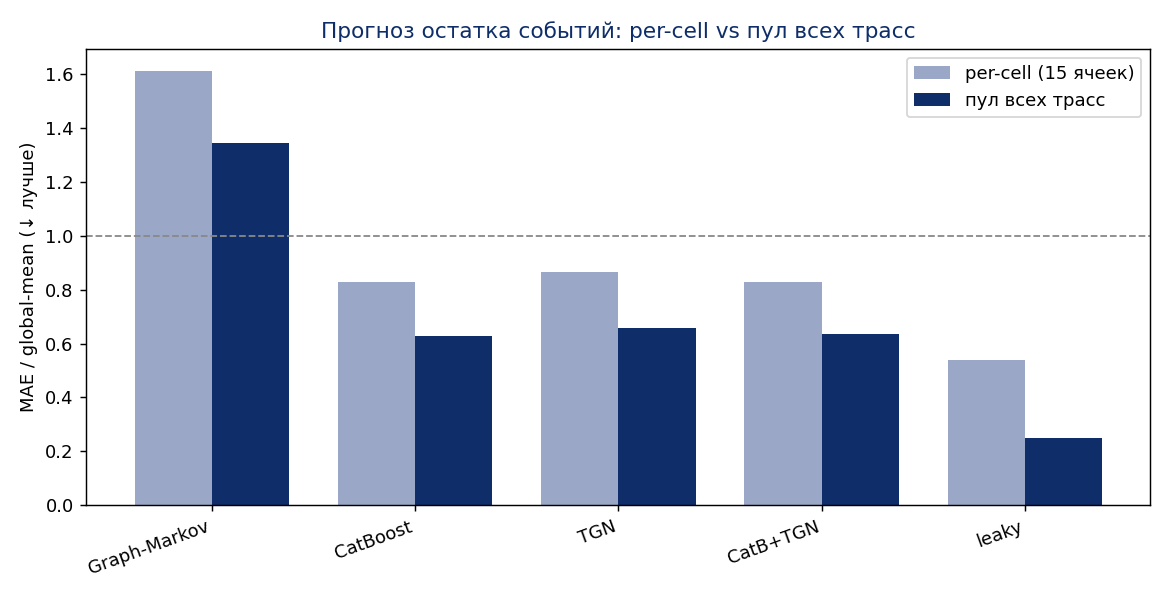
\includegraphics[width=0.8\textwidth]{fig_pool}
\caption{Обучение отдельного оценщика на каждой паре $\langle$модель$\times$бенчмарк$\rangle$ против обучения одного оценщика на всех трассах сразу. В первом случае доля объяснённой дисперсии остаётся около нуля; обучение на всех трассах с признаками модели, бенчмарка и трудности позволяет оценщику учесть различия длин между парами и уменьшает среднюю абсолютную ошибку на $35$-$37\%$.}
\label{fig:pool}
\end{figure}

\paragraph{Трудность и длина.} Готовых меток трудности нет, поэтому мы оцениваем трудность вопроса числом других моделей, ответивших на него правильно; чем больше моделей решили вопрос, тем он считается легче. Трудность связана со стоимостью: на тех парах $\langle$модель$\times$бенчмарк$\rangle$, где длина следует за трудностью, ранговая корреляция трудности с длиной равна $-0.42$, то есть более трудные вопросы получают более длинные трассы. Но сила связи зависит от бенчмарка, она высока на GPQA, HotpotQA и MuSiQue, ниже на MATH500 и на HLE практически отсутствует, там ранговая корреляция равна $-0.017$. Длина трассы плохо прогнозирует трудность вопроса, и это согласуется с наблюдением, что модель продолжает рассуждать уже после того, как ответ найден.

\section{Остановка генерации без изменения весов модели}
\label{sec:nolearn}

Остановка после заранее заданного числа токенов не меняет весов модели. Более сложный контроллер может оценивать уже написанную часть трассы и завершать рассуждение при пересечении выбранного порога. Мы проверили два таких контроллера на $244$ отложенных вопросах gpt-oss-20b: $100$ из MATH500, $40$ из GPQA-diamond и $104$ из HLE. Постоянные ограничения и правила по прогнозу применялись к одним и тем же исходным трассам и использовали один механизм принудительного перехода к финальному ответу.

\paragraph{Прогноз остатка по внутренним сигналам модели.} Этот опыт выполнен только на gpt-oss-20b. В сохранившихся трассах Qwen и Gemma распределения следующего токена не записывались, поэтому приведённые ниже числа не подтверждают переносимость результата на другие модели. Детектор событий представляет трассу последовательностью позиций и типов событий. Модель прогноза использует из этого представления число событий каждого типа, накопленное к выбранной позиции. Добавление этих счётчиков к позиционным признакам не меняет качество прогноза остатка: доля объяснённой дисперсии равна $0.590$ с ними и без них, а лучший прогноз полного расхода по событиям достигает $0.703$. Поэтому мы отдельно проверяем величины, которые модель вычисляет на каждом токене. По форме распределения вероятностей следующего токена видно, насколько модель уверена в продолжении. Мы берём семь величин, посчитанных на каждом шаге генерации: энтропию распределения, дисперсию информационного содержания, неожиданность фактически выбранного токена, вероятность самого вероятного кандидата, отрыв первого кандидата от второго, логарифм ранга выбранного токена и расхождение распределения с распределением предыдущего шага. Эти семь величин мы пропускаем через однослойную рекуррентную сеть, которой на каждом шаге доступно только прошлое, и прогнозируем две величины: сколько событий и сколько токенов трассе осталось. На отобранной подвыборке из $616$ трасс доля объяснённой дисперсии полного расхода равна $0.78$ для рекуррентной сети по распределению следующего токена и $0.70$ для градиентного бустинга по счётчикам событий. Полные результаты приведены в табл.~\ref{tab:monitor}. Скрытые состояния модели не дают ничего сверх дешёвых величин, посчитанных по распределению следующего токена, так что их дорогая выгрузка не оправдана. Отдельная маленькая языковая модель, читающая только текст трассы и не имеющая доступа внутрь основной модели, почти догоняет модель прогноза по внутренним сигналам и даёт $0.76$, то есть большая часть сигнала уже содержится в наблюдаемом тексте. Предобучение сети на вспомогательной задаче разметки фаз рассуждения переносится на прогнозирование расхода и даёт лучший результат по полному расходу.

\begin{table}[t]
\centering
\begin{tabular}{lccc}
\toprule
вход модели прогноза & P1 $R^2\uparrow$ & P2 $R^2\uparrow$ & P2 MAE$\downarrow$ \\
\midrule
счётчики событий, лучший из двух оценщиков & $0.590$ & $0.703$ & $697$ \\
распределение следующего токена & $0.598$ & $\mathbf{0.776}$ & $647$ \\
скрытые состояния               & $0.557$ & $\mathbf{0.776}$ & $636$ \\
оба входа вместе                & $0.589$ & $0.769$ & $659$ \\
текст трассы, малая языковая модель & $0.628$ & $0.760$ & $659$ \\
\midrule
\multicolumn{4}{l}{роль предобучения на входе из распределения следующего токена, P2 $R^2$:}\\
предобучение заморожено / с нуля / целиком дообучено & \multicolumn{3}{c}{$0.776$ / $0.761$ / $0.735$}\\
\bottomrule
\end{tabular}
\caption{Прогноз по внутренним сигналам модели против оценщиков по счётчикам событий. Выборка: $616$ трасс gpt-oss-20b в математическом домене, из них $279$ с HLE, $239$ с MATH500 и $98$ с GPQA-diamond. Вопросы поделены между обучением и оценкой пополам с фиксированным начальным значением генератора, $305$ против $311$, и на каждой трассе взято по три позиции наблюдения, всего $933$ проверочных точки. Эти числа получены отдельно от прогонов оценки политик и на другую выборку не переносятся. Столбец P1 отвечает прогнозу числа оставшихся событий, столбцы P2 прогнозу полного расхода трассы в токенах; $R^2$ есть доля объяснённой дисперсии, MAE средняя абсолютная ошибка в токенах. Строка сравнения даёт лучший из двух оценщиков по счётчикам событий, гребневой регрессии для P1 и градиентного бустинга для P2. Скрытые состояния не превосходят величин, посчитанных по распределению следующего токена, а текст без доступа внутрь модели почти догоняет их.}
\label{tab:monitor}
\end{table}

\paragraph{Позиции проверки задавались регулярной сеткой, а не процессом Хоукса.} На одной выборке из $244$ вопросов мы проверили два отдельных контроллера. Первый был логистической регрессией, обученной прогнозировать, снизит ли принудительное завершение в текущей позиции правильность итогового ответа. В её признаки входили агрегаты семи величин из распределения следующего токена, накопленные счётчики шести типов событий и сведения о том, была ли в уже написанной части сформулирована версия ответа. Второй контроллер использовал рекуррентную модель прогноза из предыдущего параграфа. При применении ему были доступны только семь величин из распределения следующего токена, по которым он оценивал среднее и квантили полного расхода. Событийная разметка входила в признаки первого контроллера и использовалась для вспомогательного предобучения второго, но позиции проверки в обоих случаях оставались регулярными. Оценённые параметры процесса Хоукса не использовались ни в признаках, ни при выборе позиций, ни в правиле остановки.

\paragraph{Проверенные пороговые правила не превзошли постоянные ограничения на одной выборке.} Логистический контроллер завершал рассуждение, когда оценённая вероятность безопасной остановки превышала порог. Для рекуррентной модели прогноза мы проверили два семейства правил: остановку после достижения выбранной доли прогнозируемого полного расхода и остановку при малом прогнозируемом остатке. Во всех случаях контроллер дописывал служебный токен конца размышления и запускал генерацию финального ответа. Постоянные ограничения использовали тот же механизм. Ни одно правило по прогнозу не дало одновременно не меньшую долю правильных ответов и меньший средний расход, чем постоянные ограничения на тех же трассах. Одно из постоянных ограничений сохранило долю правильных ответов прогона без ограничения и примерно вдвое сократило среднее число токенов. Этот результат получен на одной модели, одном разбиении и одной жадно сгенерированной трассе на вопрос. Контроллеры, которые выбирают позиции проверки по событиям или состоянию процесса Хоукса, в этом опыте не проверялись.

\paragraph{Переигровка с истинным остатком вместо прогноза.} Отрицательный результат мог означать слабость модели прогноза, поэтому мы переиграли те же правила по сохранённым трассам, подставив вместо прогноза истинный полный расход и истинный остаток, известные задним числом. Популяция состояла из $192$ вопросов, у которых прогон без ограничения завершился; $52$ самых длинных вопроса в неё не попали, что смещает выборку к коротким трассам. Даже при идеальном знании будущего остановка на выбранной доле собственного расхода и остановка при малом остатке не приблизились к фронту постоянных ограничений: лучшая из них даёт $0.495$ при $2849$ токенах против $0.505$ при $935$ у постоянного ограничения. Причина в устройстве самих правил: они тратят долю длины каждой трассы и наследуют тяжёлый хвост распределения длин, тогда как постоянное ограничение этот хвост обрезает. Отрицательный результат контроллеров объясняется, стало быть, конструкцией проверенных семейств правил, а не качеством модели прогноза. Запас нашёлся у другого семейства: правило, останавливающееся на самом раннем срезе, где принудительно сформулированный ответ уже правилен, даёт $0.547$ при $438$ токенах и превосходит весь фронт постоянных ограничений. Ценность остановки лежит не в прогнозе остатка, а в определении момента, когда ответ уже готов; именно это мотивирует бейзлайн по уверенности модели в ответе. Сетки срезов при этом разрежены, а ранний правильный срез включает случайные угадывания, поэтому $0.547$ при $438$ есть верхняя граница, а не достижимая точка. Прямая проверка бейзлайна по уверенности выполнена на полном банке из $788$ принудительных финалов на тех же $244$ вопросах: правило, останавливающееся при высокой средней лог-вероятности токенов принудительного финала, не превзошло постоянные ограничения ни на одном пороге, его лучшая точка даёт $0.406$ при $1146$ токенах против $0.459$ при $1034$ у ограничения $2048$; сигнал по первому токену ответа ещё слабее. Потолок раннего правильного ответа существует, но средняя уверенность финала его не реализует, и поиск доступного сигнала готовности ответа остаётся открытой задачей.

\paragraph{Уровень усилий в системном запросе.} Шаблон запроса gpt-oss содержит поле уровня усилий рассуждения со значениями low, medium и high; во всех остальных прогонах этой работы использовано значение по умолчанию medium. Смена значения есть ещё одно правило без обучения. В одном прогоне жадной оценки на $140$ отложенных вопросах при ограничении $3072$ замороженная база даёт $0.636$ при $253$ токенах на low, $0.621$ при $879$ на medium и $0.543$ при $1572$ на high. Значение low сокращает расход базы в $3.5$ раза без потери доли правильных ответов, а значение high под этим ограничением вредит из-за обрывов. Эффект обучения этим полем не воспроизводится: обученные политики в том же прогоне дают на low и medium $0.736$-$0.786$, выше любой базовой точки. Поле и обучение сочетаются: политика, обученная при medium, на low сохраняет свою долю правильных ответов при $169$ токенах. Базовые числа этого прогона ниже, чем в главной таблице: жадная генерация vLLM не воспроизводится между запусками, а уточнённый разбор финальных блоков к этому прогону не применялся, поэтому сравнения здесь ведутся только внутри одного прогона; правило сопоставления прогонов описано в разделе~\ref{sec:rl}.

\paragraph{Направления остановки и прогноза расхода различаются.} В отдельной проверке выходного слоя gpt-oss-20b косинус между направлением, которое повышает вероятность завершить рассуждение, и направлением, из которого линейная модель восстанавливает остаток расхода, равен $0.08$-$0.19$. Это соответствует углу около восьмидесяти градусов. По первому направлению близость конца трассы почти не восстанавливается. Соседний сигнал раннего выхода предлагает SpecExit, где решение о выходе подсказывает лёгкая спекулятивная модель \citep{yang2025specexit}; наш отрицательный результат с прогнозом остатка этот сигнал не покрывает.

\section{Награда за краткость при правильном ответе}
\label{sec:rl}

\paragraph{Функция награды и фактически оптимизированная цель.} Для вопроса $x$ и уже написанной части ответа $y_{<t}$ модель задаёт распределение вероятностей следующего токена $\pi_\theta(y_t\mid x,y_{<t})$. Совокупность таких распределений для всех возможных префиксов дальше называем политикой, а один сгенерированный ответ на вопрос называем роллаутом. Пусть $v(y)$ обозначает наличие непустого разобранного финального ответа, $c(y)$ его правильность, а
\begin{equation}
\ell(y)=\min\{\max(L(y),16)/L_{\max},1\}.
\label{eq:grpo-len}
\end{equation}
В основных прогонах использованы две функции награды:
\begin{align}
R_{\mathrm{all}}(x,y)
  &=\mathbf{1}[v(y)\wedge c(y)]-\lambda\,d(y)+q(y),
  &d(y)&=
  \begin{cases}
  1,& \neg v(y),\\
  \ell(y),& v(y),
  \end{cases}
\label{eq:grpo-reward}\\
R_{\mathrm{gate}}(x,y)
  &=\mathbf{1}[v(y)\wedge c(y)]
    +\lambda\,\mathbf{1}[v(y)\wedge c(y)](1-\ell(y))+q(y).
\label{eq:grpo-gate}
\end{align}
Здесь $L(y)$ есть длина рассуждения в токенах, $L_{\max}=3072$, а $q(y)$ равен $-1$ при отсутствии валидного финала, $-1/2$ при финальном блоке длиннее $256$ токенов и нулю иначе. Первая форма при $\lambda=0.3$ штрафует длину каждого валидного ответа, включая неправильный, и назначает невалидному ответу максимальную стоимость длины. Вторая форма при $\lambda=0.1$ начисляет премию за краткость только правильному валидному ответу. Нижний порог $16$ не запрещает короткое рассуждение, а прекращает дальнейший рост премии ниже этой длины. Правильность проверяется автоматически: на MATH500 по нормализованному ответу, на GPQA-diamond по выбранному варианту.

На вопрос $x$ генерируется группа из $G=8$ роллаутов. Награда каждого роллаута преобразуется в групповое относительное преимущество:
\begin{equation}
\hat A_i=\frac{R(x,y_i)-\tfrac1G\sum_j R(x,y_j)}{\mathrm{std}_j\,R(x,y_j)+\varepsilon},
\label{eq:grpo-adv}
\end{equation}
а основные прогоны минимизируют нормированную по числу токенов цель
\begin{equation}
\mathcal L(\theta)=
\frac{1}{\sum_i |y_i|}
\sum_i\left[
  -\hat A_i\sum_t\log\pi_\theta(y_{it}\mid x_i,y_{i,<t})
  +\beta\sum_t\left(e^{z_{it}}-z_{it}-1\right)
\right],
\label{eq:grpo-obj}
\end{equation}
где $z_{it}=\log\pi_{\mathrm{ref}}(y_{it}\mid x_i,y_{i,<t})-\log\pi_\theta(y_{it}\mid x_i,y_{i,<t})$. Второе слагаемое представляет собой неотрицательную оценку расхождения с замороженной базой. Групповая нормировка награды в \eqref{eq:grpo-adv} взята из GRPO \citep{shao2024deepseekmath,deepseekr1}. Первое слагаемое в \eqref{eq:grpo-obj} есть базовое правило градиента политики: при положительном $\hat A_i$ оно повышает вероятности токенов ответа, а при отрицательном понижает. В формуле используются только вероятности при текущих весах $\theta$. Вероятности тех же токенов, сохранённые при генерации роллаута политикой $\pi_{\mathrm{old}}$, в эту цель не подставляются. Они используются только в сравниваемых ниже способах обновления. В коде у этого варианта исторически стоит метка \texttt{a2c}, но это не алгоритм A2C \citep{mnih2016a3c}: обучаемого критика в наших прогонах нет. Обучаются надстройки LoRA ранга $16$ на матрицах внимания q, k, v и o. Роллауты генерирует отдельный процесс vLLM. Пробный прогон на $20$ обновлений проверил связку генерации, разбора, награды и оптимизатора: доля пустых рассуждений и переполненных финальных ответов осталась нулевой, а средняя оценка расхождения с базой не превысила $0.002$.

\paragraph{Разбор финальных блоков и правило сопоставления прогонов.} Финальный ответ извлекается из служебного блока в тексте генерации. Модель gpt-oss в $3$-$6\%$ трасс дописывает к имени этого блока служебный маркер ограничения формата; первоначальный разбор такие блоки не распознавал, и вопрос засчитывался как оставшийся без ответа. Награда отучает обученные политики от редких форм заголовка, поэтому такие блоки порождают только необученная база и политики, почти не отошедшие от неё. Все числа прогонов vLLM в этой статье пересчитаны по сохранённым дампам с уточнённым разбором; эталонная оценка при ограничении $8192$ и срез HLE сохранили тексты не полностью, и к ним пересчёт ещё не применён, что оговорено на месте. Отдельное свойство обвязки: жадная генерация vLLM с пакетной обработкой не воспроизводится между запусками, доля правильных ответов базы по четырём прогонам одного протокола лежит в $0.68$-$0.72$ с уточнённым разбором, поэтому числа сравниваются только внутри одного прогона vLLM. Побайтово воспроизводится лишь эталонная обвязка с генерацией по одному ответу на одном типе карты, и она служит опорой подтверждающих сравнений.

\paragraph{Сокращение расхода и рост доли правильных ответов на отложенной выборке.} За $100$ итераций длина сэмплированных роллаутов на обучающих промптах падает с $889$ до $431$ токена в прогоне с базовым правилом и $128$ роллаутами на итерацию. Это измерение на обучающих задачах; основные числа ниже получены жадной генерацией на невиданных вопросах. На отложенной выборке из $140$ вопросов обе основные политики дают большую долю правильных ответов и меньший средний расход, чем замороженная модель. Для модели со штрафом за длину каждого ответа доля правильных ответов растёт с $0.729$ до $0.814$, разность на одних и тех же вопросах равна $0.086$ с $95\%$ бутстреп-интервалом от $0.029$ до $0.150$. На $16$ вопросах обученная модель ответила правильно, а замороженная ошиблась; на $4$ вопросах произошло обратное, критерий Макнемара даёт $p=0.012$. Средний расход снижается с $879$ до $355$ токенов, разность на одних и тех же вопросах равна $-524$ с интервалом от $-671$ до $-386$. Для варианта, в котором краткость вознаграждается только при правильном ответе, доля правильных ответов также равна $0.814$, интервал прироста составляет от $0.036$ до $0.143$. На $14$ вопросах обученная модель ответила правильно при ошибке замороженной, обратное произошло на двух вопросах, $p=0.0042$. Средний расход этого варианта снижается до $474$ токенов, интервал разности составляет от $-547$ до $-273$. На MATH500 и GPQA-diamond знаки обеих разностей совпадают. Внутри этого прогона у обеих политик с $95\%$ уверенностью доля правильных ответов выше, а расход ниже, чем у базы.

\begin{table}[t]
\centering
\begin{tabular}{lcc}
\toprule
политика, отложенная выборка $n{=}140$ & \shortstack{доля правильных\\ответов} & токены \\
\midrule
замороженная база                        & $0.729$ & $879$ \\
GRPO с базовым правилом, $\lambda{=}0.3$                     & $0.814$ & $355$ \\
GRPO с базовым правилом и условием правильности, $\lambda{=}0.1$ & $0.814$ & $474$ \\
GRPO с базовым правилом, отставание $2$ & $0.757$ & $358$ \\
GSPO, среднее по последовательности & $0.750$ & $912$ \\
\bottomrule
\end{tabular}
\caption{Награда за краткость при правильном ответе, отложенная выборка $n{=}140$, единый жадный протокол оценки. Все строки взяты из одного процесса vLLM на одной карте и пересчитаны уточнённым разбором финальных блоков; парные интервалы и критерий Макнемара приведены в тексте. Основные политики превосходят замороженную базу по обеим величинам внутри этого запуска.}
\label{tab:grpo}
\end{table}

\paragraph{Тип GPU изменяет результат жадной генерации.} Перед подтверждающими сравнениями мы трижды оценили один и тот же адаптер на тех же $140$ вопросах при ограничении $3072$. Эталонный режим генерировал ответы по одному через Transformers при нулевой температуре. Два запуска на A100 совпали по правильности, числу токенов и извлечённому ответу на всех вопросах: доля правильных ответов равна $0.7857$, средний расход $327.5$ токена, доля валидных финалов $1.000$. Запуск на H200 сохранил ту же итоговую долю правильных ответов, но изменил правильность на $14$ вопросах, извлечённый ответ на $24$ и число токенов на $101$; средний расход вырос до $370.4$ токена, а доля валидных финалов снизилась до $0.979$. Одинаковая итоговая доля правильных ответов между картами не означает воспроизводимости, поскольку состав решённых вопросов различается. Эта проверка не заменяет парное сравнение в табл.~\ref{tab:grpo}, поскольку замороженная база в ней не оценивалась. Она устанавливает другое: тип карты входит в условия оценки, и подтверждающие сравнения должны выполняться на одном типе GPU.

\paragraph{Разбиение вопросов и механизм роста доли правильных ответов.} Обучающая часть содержит $558$ вопросов, отложенная $140$, а пересечение пусто по идентификатору и нормализованному тексту. Число итераций заранее равно ста, поэтому состояние модели по отложенной выборке не выбиралось. Эти две проверки исключают прямое совпадение вопросов и выбор наиболее удачного промежуточного состояния, но не заменяют проверку на новых корпусах и при других начальных значениях генератора. Для подтверждающей оценки до запуска зафиксирована новая выборка из $510$ вопросов: $90$ задач AIME, $260$ MMLU-Pro и $160$ BBH. Эти корпуса не участвуют в обучении; пересечений с обучающей и настроечной частями нет по идентификатору, нормализованному тексту, близости текстов с порогом $0.7$ и совпадению вопроса вместе с ответом. Выборка из $510$ вопросов не участвовала ни в одном обучении и ни в одной оценке. При мощности $0.80$ прежние $140$ вопросов различают парный прирост доли правильных ответов от $10.1$ процентного пункта, а $510$ вопросов от $5.5$ пункта.

Сравнение одних и тех же вопросов показывает, откуда берётся прирост. Замороженная модель даёт проверяемый финальный ответ на $121$ вопросе из $140$, модель со штрафом за длину каждого ответа на $137$, а вариант с наградой за краткость только правильного ответа на $135$. Ограничение длины исчерпывают соответственно $19$, $3$ и $6$ ответов. Модель со штрафом за длину правильно отвечает на $16$ вопросов, где замороженная модель ошибается; обратное происходит на $4$ вопросах. В $9$ из этих $16$ случаев замороженная модель вообще не даёт проверяемого финального ответа. Среди $119$ вопросов, на которые обе модели дали такой ответ, обученная модель права при ошибке замороженной на $7$ вопросах, а замороженная права при ошибке обученной на $3$; остаточный прирост равен четырём вопросам, двухсторонний точный критерий Макнемара даёт $p=0.344$. У варианта с наградой за краткость только правильного ответа обученная модель права при ошибке замороженной на $14$ вопросах, обратное происходит на двух. В $9$ из этих $14$ случаев замороженная модель не даёт проверяемого финального ответа. Среди $119$ вопросов с двумя проверяемыми финальными ответами обученная модель права при ошибке замороженной на $5$ вопросах, обратный случай один, тот же критерий даёт $p=0.219$. Следовательно, предотвращение обрывов объясняет большую часть роста доли правильных ответов, но не весь наблюдаемый прирост. Влияние награды за краткость и общего обучения завершать ответ разделяет контроль с $\lambda=0$, приведённый ниже.

\paragraph{Контроль без штрафа за длину и оценка при большом ограничении.} Мы обучили по три повтора с разными начальными значениями генератора для трёх наград: только правильность и валидность при $\lambda=0$, штраф за длину каждого ответа при $\lambda=0.3$ и премия за краткость правильного ответа при $\lambda=0.1$. Обучающая часть взята из отдельного пула повторных обучений и содержит $446$ вопросов, поэтому эти адаптеры не совпадают с адаптерами главной таблицы; неприкосновенная выборка из $510$ вопросов в этот пул не входит. Для первых двух наград обучение повторено ещё на двух разбиениях того же пула, всего $21$ обучение. Обучение только за правильность почти не сокращает расход, около $723$ токенов против $858$ у замороженной базы в том же прогоне, а его доли правильных ответов по трём повторам равны $0.764$, $0.764$ и $0.800$ против $0.757$ у базы с уточнённым разбором: прямое превышение над базой в этом прогоне лежит в пределах межповторного разброса. Вклад правильности в точность виден поэтому не из этого прямого сравнения, а из сочетания двух фактов: политики со штрафом значимо превосходят базу в главной таблице, а разность долей правильных ответов между наградами с $\lambda=0$ и $\lambda=0.3$ лежит в пределах шума, то есть сам штраф точности не добавляет. Штраф добавляет сжатие: у трёх повторов с $\lambda=0.3$ расход равен $329$-$349$ токенам. Отношение расхода к варианту $\lambda=0$, усреднённое по повторам, равно $0.468$ с $95\%$ бутстреп-интервалом по вопросам от $0.410$ до $0.532$; на настроечной части из $112$ вопросов оно равно $0.416$ с интервалом от $0.360$ до $0.476$. Разность долей правильных ответов между этими наградами лежит в пределах шума: $+0.024$ с интервалом от $-0.019$ до $+0.067$ на отложенной выборке и $-0.018$ с интервалом от $-0.066$ до $+0.027$ на настроечной. На двух дополнительных разбиениях доли правильных ответов лежат в $0.771$-$0.800$ у $\lambda=0$ и в $0.771$-$0.829$ у $\lambda=0.3$ при том же сокращении расхода. Итог: сокращение расхода даёт штраф за длину, а рост доли правильных ответов относится к обучению правильности, поскольку штраф сверх неё точности не добавляет.

Сравнение с базой при большом ограничении выполнено в эталонном режиме на одном типе карты, ответы генерировались по одному. При ограничении $8192$ база обрывается лишь на $5.7\%$ вопросов и даёт $0.736$ при $1326$ токенах. Три повтора с $\lambda=0$ дают в среднем $0.793$ при $883$ токенах, три повтора с $\lambda=0.3$ дают $0.795$ при $371$; при ограничении $3072$ те же повторы дают $0.776$ при $758$ и $0.783$ при $346$. По прежнему разбору превышение над базой, которая почти не обрывается, составляет $5.7$-$5.9$ процентного пункта. К этому прогону уточнённый разбор финальных блоков ещё не применён: у базы шесть завершившихся трасс из $140$ остались без распознанного финала, и если все они окажутся валидными правильными ответами, база поднимется не более чем до $0.779$, а превышение сократится до $1.4$-$1.6$ пункта. Превышение обученных вариантов над необрывающейся базой, стало быть, сохраняется при любом исходе пересчёта, но его величина до пересчёта не устанавливается точнее интервала от $1.4$ до $5.9$ процентного пункта. Поэтому на MATH500 и GPQA-diamond рост доли правильных ответов не сводится целиком к предотвращению обрывов; на HLE, как показано в разделе~\ref{sec:limits-scope}, улучшения на завершённых парах нет.

До отложенной оценки дошли одиннадцать адаптеров, восемь из них одновременно сокращают расход и повышают долю правильных ответов внутри того же запуска. Это согласованность вариантов, а не независимая репликация: все обучения используют одно начальное значение генератора и одно разбиение вопросов.

\paragraph{Разбиение вопросов на группы по трудности.} На отложенном срезе MATH500 из $100$ вопросов сокращение расхода не сопровождается снижением доли правильных ответов ни в одной группе трудности. Трудность мы измеряем двумя независимыми способами: числом крупных моделей, ответивших правильно, и уровнем сложности, приписанным вопросу в самом наборе MATH. В голосовании участвуют deepseek-reasoner, Qwen3.6-35B-A3B и Gemma-4-26B, а gpt-oss-20b исключён, поскольку политики учились на его собственных трассах. Первая шкала ведёт себя ожидаемо: по четырём группам от самой трудной к самой лёгкой доля правильных ответов замороженной базы растёт как $0.00$, $0.33$, $0.57$, $0.92$. Средний расход базы по тем же группам равен $1630$, $1850$, $1582$ и $384$ токенам, то есть на лёгкой группе он вчетверо ниже, чем на трёх трудных, где держится в пределах $1580$-$1850$. Выигрыш сосредоточен в трудных группах обеих шкал, что и сведено в табл.~\ref{tab:difficulty}. Дальше речь о политиках, которые обучились: три варианта GSPO не обучились вовсе, их расхождение с базовой политикой равно $0.001$. У обучившихся политик на $29$ вопросах пятого уровня доля правильных ответов выше базы на $0.10$-$0.17$, а расход ниже на $500$-$650$ токенов; исключения составляют Kimi k1.5, у которого экономия всего $197$ токенов, и GSPO, у которого расход даже вырос на $7$ токенов. На $14$ вопросах, решённых правильно двумя крупными моделями из трёх, доля правильных ответов у обучившихся политик выше базы на $0.14$-$0.36$, а расход ниже на $800$-$1055$ токенов. На лёгкой группе из $79$ вопросов доля правильных ответов почти не меняется, потому что база там уже даёт $0.92$. Вопросы, проигранные после сжатия, встречаются. У трёх политик каждый такой вопрос отвечен на более короткой трассе, чем у базы, это варианты без поправки при отставании $0$ и $8$ и ограничение на отдельный токен. У обучившихся политик проигранных от одного до четырёх против девяти или десяти выигранных; у варианта без поправки при отставании $2$ проигранных пять, а у GSPO шесть проигранных против семи выигранных. Знаковый тест без поправки на множественность даёт $p$ от $0.021$ до $0.039$ у трёх политик: это $\lambda{=}0.3$, $\lambda{=}0.1$ с условием правильности и вариант без поправки при отставании $0$. С предыдущей тройкой этот список пересекается лишь в одной политике. Разрешающей способности хватает не везде: в самой трудной группе всего четыре вопроса, которые не решает ни база, ни одна политика, так что различить их там нечем; основную массу таких вопросов даёт HLE, и этот срез обсуждается в разделе~\ref{sec:limits-scope}. Числа этого разбора получены до уточнения разбора финальных блоков; спасённые уточнением вопросы базы лежат в лёгких группах MATH500, поэтому выигрыш в трудных группах они не затрагивают.

\begin{table}[t]
\centering
\begin{tabular}{lcccc}
\toprule
 & \multicolumn{2}{c}{уровень MATH} & \multicolumn{2}{c}{решивших крупных} \\
\cmidrule(lr){2-3}\cmidrule(lr){4-5}
политика & 4 ($n{=}21$) & 5 ($n{=}29$) & 2 ($n{=}14$) & 3 ($n{=}79$) \\
\midrule
$\lambda{=}0.3$ & $+0.10$ / $-485$ & $+0.17$ / $-599$ & $+0.36$ / $-950$  & $+0.04$ / $-192$ \\
$\lambda{=}0.1$ с условием правильности & $+0.14$ / $-299$ & $+0.14$ / $-506$ & $+0.29$ / $-817$  & $+0.04$ / $-156$ \\
без поправки, отставание $0$ & $+0.10$ / $-531$ & $+0.14$ / $-569$ & $+0.21$ / $-899$  & $+0.05$ / $-192$ \\
без поправки, отставание $8$ & $+0.05$ / $-610$ & $+0.10$ / $-648$ & $+0.14$ / $-953$  & $+0.05$ / $-206$ \\
DAPO, отставание $2$ & $+0.14$ / $-515$ & $+0.10$ / $-552$ & $+0.21$ / $-850$  & $+0.03$ / $-157$ \\
\bottomrule
\end{tabular}
\caption{Изменение доли правильных ответов и среднего числа токенов относительно замороженной базы по группам трудности; отложенный срез MATH500, $100$ вопросов, тот же прогон оценки, что и в остальных таблицах, разбор финальных блоков прежний. Разбиение сделано по двум разным шкалам трудности: слева уровень сложности, приписанный вопросу в самом наборе задач, справа число крупных моделей, ответивших правильно. Всего в разбор вошли девять политик, дошедших до отложенной оценки; в таблице показаны пять из них, а линия GSPO представлена одним вариантом. Ячейка читается как прирост доли правильных ответов и изменение расхода на одних и тех же вопросах. У всех пяти показанных политик доля правильных ответов растёт в обеих трудных группах, а на лёгкой группе база уже даёт $0.92$, и там меняется главным образом расход.}
\label{tab:difficulty}
\end{table}

\paragraph{Обучение при разных уровнях усилий.} Уровень усилий в запросе меняет стартовое распределение длин, поэтому мы проверили, нужна ли отдельная политика под каждый уровень. Политика, обученная при medium, переносится на low без потери доли правильных ответов, но при high теряет: в одном прогоне оценки она даёт $0.786$ при $394$ токенах на medium и $0.636$ при $1241$ на high. Обучение, в котором уровень усилий выбирается случайно для каждого обучающего запроса, даёт одну политику, устойчивую на всех трёх уровнях: $0.750$ при $162$ токенах на low, $0.786$ при $332$ на medium и $0.764$ при $784$ на high. Отдельная политика под каждый уровень не потребовалась.

\paragraph{Сравнение способов обновления весов.} Для каждого токена сгенерированного ответа берётся отношение вероятности, которую даёт ему обновляемая модель, к вероятности, которую давала модель в момент генерации: $\rho_t=\pi_\theta(y_t)/\pi_{\mathrm{old}}(y_t)$. Базовое правило из \eqref{eq:grpo-obj} не использует $\rho_t$. Остальные проверенные правила вводят это отношение и различаются тем, как взвешивают градиентный член последовательности с преимуществом $\hat A$. В PPO \citep{schulman2017ppo} отношение $\rho_t$ ограничивают сверху и снизу для каждого токена отдельно; в DAPO \citep{yu2025dapo} верхнюю и нижнюю границы выбирают раздельно. В CISPO \citep{minimax2025m1} ограниченное отношение не пропускает через себя градиент, за счёт чего ни один токен не выпадает из обучения. В GSPO \citep{zheng2025gspo} отдельные отношения заменены их геометрическим средним по всей последовательности, $s=\exp(\frac1{|y|}\sum_t\log\rho_t)$, и ограничивается уже оно. В Kimi k1.5 \citep{kimi2025k15} вместо ограничения добавлен квадратичный штраф. В SAPO \citep{gao2025sapo} и SSPO \citep{sspo2026} жёсткие границы заменены гладким изменением веса. Смещения агрегации наград по длине ответа в целях этого семейства разобраны в Dr.~GRPO \citep{liu2025drgrpo}; наша цель \eqref{eq:grpo-obj} нормирует сумму по общему числу токенов батча. Перемножение отношений по всей последовательности мы не используем из-за дисперсии, которая растёт экспоненциально с длиной. До полного прогона с отложенной оценкой мы довели не всё семейство: CISPO, SAPO и SSPO остановились на коротких проверочных запусках по десять итераций, поэтому в табл.~\ref{tab:po} сведены только правила с полным прогоном на одном протоколе оценки.

Первый из трёх наблюдаемых исходов: поправки почти не срабатывают. Обучение лёгких адаптеров LoRA меняет модель очень слабо, и вероятности, которые она приписывает токенам, сдвигаются мало: средний $|\log(\pi_\theta/\pi_{\mathrm{old}})|$ равен $0.022$ на токен. В функции обучения PPO сравнивают два значения. Первое рассчитывают с $\rho_t$, второе с копией $\rho_t$, ограниченной диапазоном от $0.8$ до $1.2$, и из них выбирают меньшее. В DAPO верхняя граница равна $1.28$. Фактическое и ограниченное отношения различаются менее чем для двух процентов токенов. В среднем по итерациям с $80$ по $100$ награда равна $0.659$ у базового правила, $0.649$ у PPO и $0.666$ у DAPO, поэтому ограничение отношений не создаёт отдельного режима обучения в этих прогонах.

Второй исход: поправка блокирует обучение. Геометрическое среднее отношений вероятностей по всей последовательности замораживает политику на уровне базы, и абляция показывает, что опубликованный порог ограничения тут ни при чём: снятие ограничения ничего не меняет, расхождение с базой остаётся порядка $10^{-3}$, результат на отложенной выборке неотличим от замороженной модели. Причина в другом множителе: геометрическое среднее масштабирует градиент от каждого токена величиной $s/|y|$, то есть делит эффективный шаг обучения на длину последовательности, а она здесь измеряется сотнями. При неадаптированном шаге обучение с такой целью не идёт ни с ограничением, ни без него.

Третий исход: поправка обучается, но мешает цели. Квадратичный штраф за отход от прежних весов сохраняет долю правильных ответов, но оставляет длину рассуждения прежней, то есть блокирует ровно то сжатие, ради которого награда и вводилась.

Обучение и генерация могут идти одновременно. Один шаг обучения устроен так: модель сначала генерирует ответы, затем по ним считается градиент и обновляются веса. При параллельной работе генератор использует политику, которая была актуальна $S$ обновлений назад. В одном прогоне без отставания доля правильных ответов равна $0.800$ при $338$ токенах, при $S=2$ она равна $0.757$ при $358$ токенах, при $S=8$ равна $0.793$ при $332$ токенах. Среднее изменение логарифма вероятности одного токена растёт до $0.030$ против $0.022$ без отставания. Эти числа показывают, что отставание на восемь обновлений не вывело обучение из рабочей области в данном прогоне. Общий вывод об отсутствии потери требует повторов и проверки эквивалентности, поскольку чистых повторных обучений при одинаковых настройках нет.

\begin{table}[t]
\centering
\begin{tabular}{lccc}
\toprule
способ обновления весов, отложенная выборка $n{=}140$ & \shortstack{доля правильных\\ответов} & токены & KL \\
\midrule
замороженная база                & $0.729$ & $879$ &  \\
\midrule
базовое правило, отставание $0$, батч $64$ роллаута, это $\lambda{=}0.3$ & $0.814$ & $355$ & $0.038$ \\
базовое правило, отставание $0$, батч $128$ роллаутов & $0.800$ & $338$ & $0.036$ \\
базовое правило, отставание $2$, батч $128$ & $0.757$ & $358$ & $0.041$ \\
базовое правило, отставание $8$, батч $128$ & $0.793$ & $332$ & $0.044$ \\
ограничение на отдельный токен, $\epsilon{=}0.2$ & $0.771$ & $445$ & $0.019$ \\
DAPO $0.2/0.28$                  & $0.793$ & $403$ & $0.026$ \\
Kimi k1.5 $\beta{=}0.1$          & $0.736$ & $788$ & $0.003$ \\
\midrule
GSPO с опубликованным ограничением & $0.750$ & $912$ & $0.001$ \\
GSPO без ограничения & $0.743$ & $869$ & $0.001$ \\
GSPO, отставание $8$ & $0.743$ & $862$ & $0.001$ \\
\bottomrule
\end{tabular}
\caption{Способы обновления весов, отложенная выборка $n{=}140$, единый жадный протокол оценки, все строки из одного процесса vLLM на одной карте, разбор финальных блоков уточнён. В столбце токенов стоит их среднее число на рассуждение. Колонка KL взята не из оценки, а из логов обучения и усреднена по итерациям с $80$ по $100$. Две верхние строки базового правила различаются размером батча, $64$ и $128$ роллаутов на итерацию; награда, начальное значение генератора, скорость обучения и число итераций у них совпадают, но это не повторные обучения с полностью одинаковыми настройками. Разброс между повторами одного и того же обучения достигает $4$-$5$ процентных пунктов доли правильных ответов, поэтому различия строк меньше этого разброса не интерпретируются. Отдельная эталонная проверка показала полное совпадение повторов на A100 и расхождение между A100 и H200, поэтому строки из разных типов карт не объединяются. Базовое правило, PPO и DAPO попадают в одну область доли правильных ответов и расхода, среднее по последовательности сохраняет результат на уровне замороженной базы при любом проверенном отставании генерации, квадратичный штраф обучается, но длину не сжимает.}
\label{tab:po}
\end{table}

\paragraph{Предельное сжатие без обучения с наградой.} Более дешёвая замена обучению с наградой это дообучение на самых коротких правильных трассах самой модели, и предельную величину такого сжатия можно измерить заранее. Мы генерируем по восемь трасс на вопрос и сравниваем самую короткую правильную трассу с типичной правильной. Модель регулярно решает задачу заметно короче, чем делает это обычно: на решаемых вопросах кратчайшая правильная трасса короче типичной правильной на $35\%$ по медиане, на GPQA на $42\%$, на уже почти насыщенном MATH500 на $32\%$; всё это сведено в табл.~\ref{tab:sft}. Верхнюю границу здесь задаёт доля вопросов, которые модель вообще решает: на HLE она равна шести процентам, и сжимать там почти нечего.

\begin{table}[t]
\centering
\begin{tabular}{lcccc}
\toprule
бенчмарк & pass@1 & кратч.\,прав. & типичн.\,прав. & экономия \\
 & & токены & токены & медиана \\
\midrule
MATH500 & $0.90$ & $178$  & $270$  & $32\%$ \\
GPQA    & $0.52$ & $692$  & $1238$ & $42\%$ \\
HLE     & $0.06$ & $1891$ & $3123$ & $39\%$ \\
\midrule
все     &        &        &        & $35\%$ \\
\bottomrule
\end{tabular}
\caption{Предельное сжатие без обучения с наградой: длина кратчайшей правильной трассы против типичной правильной, модель gpt-oss-20b. По каждому корпусу взято $53$ вопроса и по восемь сэмплов на вопрос, всего по $424$ кандидата на корпус; сэмплирование при температуре единица. Вопросы взяты из обучающего пула, а не из отложенной выборки, поэтому с числами остальных таблиц эти напрямую не сравниваются. Столбец pass@1 даёт долю правильных ответов среди всех сгенерированных кандидатов. Медианная экономия около $35\%$ посчитана по $92$ вопросам, для которых есть хотя бы одна правильная трасса, и задаёт предельную цель дообучения на коротких трассах.}
\label{tab:sft}
\end{table}

\section{Границы применимости}
\label{sec:limits-scope}

\paragraph{Большая модель расходует больше токенов при сопоставимой доле правильных ответов на MATH500.} На одних и тех же $100$ вопросах доля правильных ответов deepseek-reasoner равна $0.910$, а у политики gpt-oss-20b с $\lambda=0.3$ равна $0.900$. Средний расход равен $1209$ и $323$ токена, медианный различается в $2.8$ раза. На полном MATH500 из $500$ вопросов неправильный ответ deepseek-reasoner обходится в среднем в $4683$ токена против $813$ у правильного; на общих $100$ вопросах это $5235$ против $811$ при девяти неправильных ответах. На HLE сравниваются разные выборки и протоколы: доля правильных ответов deepseek-reasoner равна $0.070$ на $2158$ вопросах при $5792$ токенах, у замороженной gpt-oss-20b она равна $0.077$-$0.086$ на $104$ вопросах при ограничениях $1024$ и $2048$. Эти измерения устанавливают большой расход deepseek-reasoner, но не показывают результат её обучения на краткость.

\begin{table}[t]
\centering
\begin{tabular}{lccc}
\toprule
 & \shortstack{доля правильных\\ответов} & токены в среднем & токены при ошибке \\
\midrule
\multicolumn{4}{l}{MATH500, общие $100$ вопросов отложенной выборки:}\\
deepseek-reasoner        & $0.910$ & $1209$ & $5235$ \\
gpt-oss-20b, база        & $0.860$ & $645$  & $1727$ \\
gpt-oss-20b, $\lambda{=}0.3$ & $0.900$ & $323$ & $1318$ \\
\midrule
\multicolumn{4}{l}{HLE, текстовый срез: deepseek на $n{=}2158$, gpt-oss на $n{=}104$}\\
deepseek-reasoner        & $0.070$ & $5792$ & $5972$ \\
gpt-oss-20b, лимит $1024$ & $0.077$ & $866$ &  \\
gpt-oss-20b, лимит $2048$ & $0.086$ & $1446$ &  \\
\bottomrule
\end{tabular}
\caption{Большая модель против наших политик. Верхний блок посчитан на $100$ вопросах MATH500, общих для обоих протоколов, числа gpt-oss пересчитаны уточнённым разбором финальных блоков: доля правильных ответов различается на один процентный пункт у политики и на пять у базы, а расход отличается в разы. Табл.~\ref{tab:grpo} считает те же политики на всех $140$ вопросах отложенной выборки, где средний расход выше за счёт более дорогого GPQA; оба набора чисел получены в одном прогоне оценки. Проверка сходится: $323$ токена на MATH500 и $433$ на GPQA дают $354$ на $140$ вопросах, что и есть $355$ в главной таблице. Нижний блок сводит два разных прогона на разных выборках: deepseek прогнан на текстовом срезе HLE из $2158$ вопросов, а наша замороженная модель с ограничениями длины на подвыборке из $104$ вопросов. Поэтому нижний блок измеряет расход каждого протокола, но не разность долей правильных ответов. Токены deepseek считаны его собственным токенизатором, расхождение с нашим на англоязычной математике измеряется процентами.}
\label{tab:h1}
\end{table}

\paragraph{Точки других моделей на нашем протоколе.} Старшая модель того же семейства gpt-oss-120b оценена в одном прогоне на тех же $140$ вопросах при ограничении $3072$: доля правильных ответов равна $0.786$ при $283$ токенах на уровне усилий low, $0.679$ при $707$ на medium и $0.536$ при $1337$ на high. Модель в шесть раз крупнее нашей также многословна при уровне по умолчанию и также теряет под ограничением при высоком уровне усилий. Обученные политики gpt-oss-20b достигают сопоставимой доли правильных ответов при меньшем расходе, но эти числа получены в разных прогонах, и парного сравнения здесь нет. Модель DeepSeek-R1-Distill-Llama-70B, у которой размышление выделено в тексте ответа парой служебных тегов, на том же наборе вопросов даёт $0.479$ при $606$ токенах размышления и $19\%$ обрывов; инструкция для неё помещена в пользовательское сообщение, поскольку системные запросы для этой модели не рекомендованы её авторами. Phi-4-reasoning-plus с нашим протоколом несовместима: даже при ограничении $8192$ обрывается $76\%$ ответов, проверяемый финал остаётся у $24\%$, а типичное размышление длиннее восьми тысяч токенов.

\paragraph{При восьми роллаутах HLE часто не даёт группового сигнала правильности.} На HLE доля правильных ответов замороженной модели держится на уровне $0.05$-$0.09$ при ограничениях от $256$ до $4096$ токенов, а доля обрывов меняется от $92\%$ до $38\%$. Прогон без ограничения содержит только два вопроса и не позволяет заключать, что дополнительный расход бесполезен на всём корпусе. Для обучения измерена другая конкретная проблема: среди $53$ вопросов с восемью роллаутами у $43$ нет ни одного правильного ответа. На этих $81\%$ групп компонент правильности одинаков для всех роллаутов, поэтому групповое относительное преимущество по нему равно нулю. Увеличение группы, отбор задач с ненулевой вероятностью решения или промежуточная награда представляют собой отдельные способы восстановить сигнал.

\paragraph{На HLE рост конечной точности вызван завершением ответов.} На текстовом срезе из $2{,}157$ вопросов при ограничении рассуждения $3072$ доля проверяемых финальных ответов замороженной gpt-oss-20b равна $0.539$, а у четырёх обученных вариантов лежит от $0.923$ до $0.979$. Их доля правильных ответов равна от $0.0607$ до $0.0663$ против $0.0436$ у замороженной модели, а средний расход составляет от $474$ до $833$ токенов против $2031$. Среди $1{,}147$-$1{,}160$ вопросов, на которые обе сравниваемые модели дали проверяемый финальный ответ, разность долей правильных ответов лежит от $-0.0069$ до $0.0044$, точный парный критерий даёт значения $p$ от $0.45$ до $1.00$. Наблюдаемый прирост сосредоточен в $994$ вопросах, где замороженная модель израсходовала ограничение и не дала ответа. Эти данные показывают, что обучение резко сокращает обрывы и поэтому повышает конечную точность при заданном ограничении. Улучшение способности решать уже завершённые задачи на HLE не обнаружено. Завершать ответы модель учится и без штрафа за длину: два повтора обучения при $\lambda=0$ дают на том же срезе $0.0542$ и $0.0654$, два повтора при $\lambda=0.3$ дают $0.0626$ и $0.0663$ против $0.0454$ у замороженной модели в том же прогоне. Уточнённый разбор финальных блоков к этому срезу ещё не применён; по доле трасс с маркером формата поправка к базе оценивается примерно в $0.009$ и вывода о механизме не меняет.

На GPQA замороженная модель тратит больше на ошибки: неправильный ответ обходится в $1992$ токена против $669$ у правильного, а медиана неправильного ответа равна потолку $3069$ при ограничении $3072$. Политика $\lambda=0.3$ сокращает обе величины, но сохраняет тот же порядок: $669$ токенов при ошибке против $276$ при правильном ответе. В этом прогоне модель не научилась завершать нерешаемые вопросы дешевле решаемых.

\section{Пределы тонкой структуры рассуждения}
\label{sec:labels}

Награда \eqref{eq:grpo-reward} платит за исход и за длину. Плата за процесс, то есть за то, как именно устроено рассуждение, могла бы добавить к этому что-то ещё. Мы проверили это на четырёх источниках разметки и получили в основном отрицательный ответ.

Источники таковы: разметка по текстовым шаблонам; полная переразметка $6{,}106$ трасс одной сильной моделью-судьёй; разметка ещё более сильной моделью-судьёй на $215$ математических трассах трёх моделей-источников, всего по двум доменам $427$; разметка ещё одной открытой моделью на $2{,}702$ математических трассах. Для каждого источника мы обучили одинаковый по устройству распознаватель событий, работающий по тексту трассы, чтобы его можно было дёшево вызывать прямо во время генерации роллаутов. Порог отбора мы задали заранее: распознаватель должен воспроизводить счётчики событий своей же разметки с ранговой корреляцией не ниже $0.6$. Прошли два источника из четырёх: разметка по шаблонам с корреляцией $0.99$ и разметка сильной моделью-судьёй на полном корпусе с корреляцией $0.78$. Разметка самой сильной модели не прошла из-за размера, её $215$ математических трасс дают всего $0.22$, а четвёртая не добрала до порога $0.005$, показав $0.595$.

Ни один распознаватель не переносится на чужую разметку: обученный на одной, он воспроизводит счётчики другой с ранговой корреляцией $0.05$ и $-0.08$ по двум доменам. При используемых определениях разные источники не согласуются в том, какие фрагменты текста считать событиями одного типа. Согласие на уровне отдельных событий, посчитанное как гармоническое среднее точности и полноты, равно $0.25$ и $0.30$ по двум доменам. Прямое сравнение судей уточняет природу этой непереносимости. Два сильных судьи с одинаковой инструкцией согласны между собой по счётчикам событий с ранговой корреляцией $0.745$ на $1652$ общих трассах, тогда как судья с шаблонной разметкой согласен лишь с корреляцией $0.513$; значит непереносимость шаблонного слоя есть разница определений события, а не случайный шум. На длинных плотных трассах согласие падает и между сильными судьями, до $0.121$, а сведение шести типов к четырём грубым группам почти не помогает: среднее гармоническое точности и полноты растёт с $0.36$ лишь до $0.38$. Понятие события, стало быть, устойчиво между судьями на трассах обычной плотности, шаблонное определение является другим определением, а на плотных трассах конструкт нестабилен сам по себе.

Линию моделей, оценивающих отдельные шаги решения, мы проверили на том же корпусе, и её собственный сигнал оказался слабым. Открытая модель, которая оценивает шаги с учётом всей предыдущей части трассы, оценила все $6{,}106$ трасс. На математическом срезе из $3{,}288$ трасс ранговая корреляция её оценки с правильностью ответа равна $0.257$, если по трассе брать минимальную из пошаговых оценок, $0.369$ при усреднении и $0.300$ по последнему шагу, то есть рекомендованный в литературе минимум проигрывает простому среднему. По всему корпусу из $6{,}106$ трасс сигнал ещё слабее: $0.162$ у минимума, $0.199$ у среднего и $0.283$ у последнего шага. Перенести её оценки в быстрый распознаватель по тексту не удалось, порог не пройден: корреляция ученика с учителем составила $0.44$ и $0.55$ по доменам при пороге $0.7$. Связь такого ученика с правильностью ответа равна $0.251$, ровно на уровне уже имеющегося распознавателя событий с его $0.246$.

Событийную составляющую награды мы проверили и в самом обучении. К награде \eqref{eq:grpo-reward} добавлялся член, равный отношению числа найденных распознавателем событий к целевому числу для данной длины, с потолком в единицу. С весом $0.2$ ни одна из двух прошедших порог разметок не превзошла контроль без событийного члена: в одном прогоне оценки на $140$ отложенных вопросах контроль даёт $0.807$ при $352$ токенах, вариант с разметкой судьи $0.779$ при $357$, вариант с разметкой по шаблонам $0.750$ при $678$. Контроль здесь есть отдельное обучение с той же наградой без событийного члена и другим размером батча, а не адаптер главной таблицы. Разметка по шаблонам ожидает $12.95$ события на тысячу токенов, и это требование конфликтует со штрафом за длину: политика почти не сжала рассуждение. Ослабленный вариант с весом $0.05$ и целевой плотностью $4$ события на тысячу токенов также не превзошёл контроль, $0.779$ против $0.793$ в другом прогоне. Две оговорки ограничивают этот вывод. В реализации событийный член не обнулялся на неправильных ответах, поэтому в группах без единого правильного ответа он оставался единственным источником группового преимущества и поощрял наращивание событий на нерешаемых вопросах. Кроме того, распознаватель считает события по текстовым шаблонам, которые обучаемая политика может производить сама по себе. Исправленная форма устранила оба дефекта: событийный член обнулялся на неправильных ответах, события считал распознаватель, использующий историю уже найденных событий, а целевая плотность задавалась либо фиксированной величиной в четыре события на тысячу токенов, либо медианной плотностью судейской разметки в $9.29$ события. Диагностический прогон с наградой только из событийного члена показал, что накрутки числа событий нет: среднее число событий на роллаут выросло лишь с $2.59$ до $2.65$, а нормированный плотностью член политика поднимает, сжимая текст вокруг уже имеющихся событий, то есть частично превращает его в замаскированный штраф длины. В одном новом прогоне оценки на тех же $140$ вопросах вариант с фиксированной плотностью дал $0.807$ при $334$ токенах против $0.764$ при $368$ у контроля с той же наградой без событийного члена, парная разность лежит в пределах шума. Вариант с судейской плотностью дал $0.836$ при $385$ токенах; его парная разность с контролем равна $+0.071$ с $95\%$ интервалом от $+0.021$ до $+0.129$ и $p=0.021$ при том же расходе. Это единственное обучение на каждое условие: при межповторном разбросе в $4$-$5$ процентных пунктов вывод о пользе исправленной событийной добавки требует повторов и остаётся открытым.

Из модели событий как точечного процесса критику переживают два результата. Спектральный радиус матрицы возбуждения по счётчикам событий восстановить нельзя, профиль правдоподобия по нему плоский; восстановить можно другой параметр. Если записать процесс как авторегрессию счётчиков по окнам, доля уровня активности окна, переносимая на следующее окно, складывается из двух вкладов, от наблюдённого счётчика и от условного среднего, и сумма этих двух коэффициентов играет роль ветвящегося параметра. Она равна $0.795$ с интервалом от $0.697$ до $0.853$ в математике и $0.983$ с интервалом от $0.965$ до $0.996$ в поисковом домене; для поискового домена это верхняя оценка, поскольку там вырождается случайный множитель неоднородности и вся наблюдаемая кластеризация относится на счёт возбуждения. Эта величина связана с хвостами распределения расхода: чем выше оценённая по данным способность каскада самоподдерживаться в паре $\langle$модель$\times$бенчмарк$\rangle$, тем чаще встречаются очень длинные трассы. Вероятность больших расходов приближённо убывает как степень; показатель этой степени падает с ростом способности каскада самоподдерживаться, ранговая корреляция равна $-0.69$ при $p=0.005$, а превышение разброса над средним растёт, ранговая корреляция равна $+0.67$ при $p=0.006$. Сама модель, её проверенные и непроверенные следствия и аналитическое тождество вмешательства вынесены в приложение~\ref{sec:theory}. Для управления расходом эти величины ничего не добавили: ни один проверенный контроллер и ни одна награда ими не воспользовались с выигрышем.

\section{Обсуждение и ограничения}

\paragraph{Сводка.} Для прогноза расхода достаточно дешёвых величин: числа уже потраченных токенов, накопленных агрегатов и распределения следующего токена; разбор рассуждения на типизированные шаги прогноз не улучшает. Для сокращения расхода работают простые рычаги. Заранее заданный предел длины не требует новых роллаутов или обучения и применяется прямо во время генерации; одно из постоянных ограничений сохранило долю правильных ответов прогона без ограничения и примерно вдвое сократило среднее число токенов. Уровень усилий в запросе даёт сопоставимый по силе рычаг без обучения. Правила остановки по прогнозу остатка постоянные ограничения не превзошли, и переигровка с истинным остатком показала, что дело в конструкции таких правил, а не в качестве модели прогноза; потолок остаётся только у правил, распознающих готовность ответа, но проверенное правило по средней уверенности финала этот потолок не реализовало. Изменение весов требует генерации групп роллаутов и обучения на GPU, зато награда за правильный и короткий ответ сокращает расход в разы и одновременно повышает долю правильных ответов, причём вклады разделяются: точность даёт компонент правильности, сжатие даёт штраф за длину. Рост приходится на трудные группы вопросов, а в лёгких сокращается только расход. Дообучение на кратчайших правильных трассах самой модели занимает промежуточное положение и имеет измеренный запас в $35\%$ по медиане на решаемых вопросах.

\paragraph{Разметка событий как источник погрешности.} Переразметка более тысячи трасс моделью-судьёй показывает, что разметка по текстовым шаблонам завышает счётчики от $2.7$ раза в математике до $9.1$ в поисковом домене, а по \textsf{commit} в $7.8$ раза, и при этом пропускает события признания неудачи; ранговая корреляция её счётчиков со счётчиками судьи равна $0.46$ и $0.17$ по двум доменам. Прогноз расхода к этому устойчив, поскольку опирается на то, сколько трасса уже прошла, а величины, описывающие процесс, неустойчивы: матрицы возбуждения, оценённые по разным разметкам, и способность каскада самоподдерживаться на разметке судьи оказываются меньше, а эффекты отдельных типов событий могут менять знак. Обученный распознаватель, которому засчитывается попадание в окно вокруг размеченного места, превосходит разметку по шаблонам на порядок, гармоническое среднее точности и полноты, усреднённое по шести типам, равно $0.40$ против $0.036$, и его счётчики воспроизводят разметку с ранговой корреляцией $0.781$ на $3{,}288$ математических трассах, чего достаточно для вызова прямо во время генерации роллаутов. Но, как мы показываем в разделе~\ref{sec:labels}, между разметками переносимости нет, поэтому любое утверждение о процессе рассуждения несёт погрешность того, кто размечал.

\paragraph{Ограничения.} (i) Стоимость мы измеряем только токенами, поэтому не измеряем напрямую денежные затраты, расход энергии и время ответа; для поискового домена задержку вызова поиска надо моделировать отдельно. (ii) Обученная политика оценена на одной модели с $20$ миллиардами параметров и на двух бенчмарках, где правильность проверяется автоматически. (iii) Контроль с $\lambda=0$ и оценка при ограничении $8192$ выполнены и разделили вклады: рост доли правильных ответов даёт обучение правильности, сокращение расхода даёт штраф за длину. Окончательная выборка из $510$ вопросов ещё не открывалась, итоговые интервалы будут посчитаны на ней. (iv) Разбор финальных блоков уточнён после основных прогонов: числа прогонов vLLM пересчитаны по сохранённым дампам, а эталонная оценка при ограничении $8192$ и срез HLE ждут пересчёта, поэтому превышение над необрывающейся базой указано интервалом от $1.4$ до $5.9$ процентного пункта. (v) Сравнение одиннадцати способов обновления весов по-прежнему использует одно начальное значение генератора и одно разбиение. Главный контраст наград повторён на трёх начальных значениях и трёх разбиениях; разброс между повторами при одинаковой награде достигает $4$-$5$ процентных пунктов доли правильных ответов, поэтому одиночные обучения не сравниваются между собой без повторов. (vi) Количественная часть событийной модели ограничена: спектральный радиус по счётчикам не восстанавливается, а формула на бесконечный горизонт завышает расход. Модель сохраняется ради проверяемых конечногоризонтных прогнозов и тождества вмешательства, а не как объяснение награды. (vii) В самой трудной группе MATH500 всего четыре вопроса, поэтому разбор по трудности не заменяет более крупную подтверждающую выборку. (viii) Распределение расхода между задачами дано как математическое предложение и не проверено на обслуживаемой группе запросов. (ix) Даже при нулевой температуре смена типа GPU меняет отдельные ответы и их длину, поэтому сравнения между запусками допустимы только при зафиксированном типе карты. (x) Контроллеры остановки проверены только на gpt-oss-20b, одном разбиении и регулярной сетке позиций; правила по событиям, состоянию процесса Хоукса и другим моделям требуют отдельного опыта. (xi) Правило остановки может чаще обрывать запросы, которым действительно нужны длинные трассы. Все использованные трассы получены как ответы моделей на пяти публичных бенчмарках, человеческие и персональные данные не использовались, поэтому этот риск не проверен на группах реальных пользователей и других типах запросов. Практическое распределение общего бюджета требует минимального гарантированного числа токенов на каждый запрос и отдельной оценки групп с длинными трассами.

\section{Заключение}

Остаток расхода прогнозируется по уже написанной части трассы, и для этого хватает дешёвых величин: числа потраченных токенов, накопленных агрегатов и распределения следующего токена. Проверенные правила остановки по этому прогнозу не превзошли постоянные ограничения, и переигровка с истинным остатком показала, что это свойство самих правил, а не модели прогноза; потолок остаётся у правил, распознающих готовность ответа, однако правило по средней уверенности финала его не реализовало. Изменение весов даёт другой результат: на $140$ отложенных вопросах две политики gpt-oss-20b повышают долю правильных ответов с $0.729$ до $0.814$ и сокращают средний расход с $879$ до $355$ и $474$ токенов. Сравнение с обучением при $\lambda=0$ и с замороженной моделью при большом ограничении выполнено на нескольких начальных значениях и разбиениях: рост доли правильных ответов даёт обучение правильности, сокращение расхода даёт штраф за длину, и при ограничении $8192$ обученные варианты сохраняют превышение над почти не обрывающейся базой. Тонкая структура рассуждения этот результат устойчиво не улучшила: типы событий не добавили к прогнозу, обученный момент остановки не превзошёл постоянные ограничения, параметры процесса Хоукса не идентифицируются по счётчикам, разметки событий не переносятся между источниками, процессные награды не связаны с правильностью сильнее готового распознавателя, а событийная добавка к награде в первоначальной форме проиграла контролю; её исправленная форма с судейской плотностью дала выигрыш в единственном обучении и ждёт повторов. Окончательная выборка из $510$ новых вопросов ещё не открывалась; на ней будут посчитаны итоговые интервалы главного сравнения.

\appendix

\section{Взаимовозбуждение типов событий}
\label{app:hawkes}

Чтобы описать, как состояние трассы меняется по ходу генерации, мы выделяем в ней события разных типов: возврат к предыдущему шагу, проверку промежуточного результата, фиксацию ответа и другие. Время события задаём его позицией в токенах от начала трассы, а тип указывает, что именно в этой позиции сделала модель. Интенсивностью события называем текущую частоту его появления с учётом уже написанной части трассы. Как показывает анализ построенных нами трасс, события обладают свойством самовозбуждения. Они идут сериями: появление одного события на некоторое время повышает интенсивность последующих. Многомерный процесс Хоукса \citep{hawkes1971,hawkes1974cluster} описывает этот механизм с отдельной интенсивностью для каждого типа события и связями между типами. Повышенную частоту очень длинных трасс мы связываем с тем, что самовозбуждение поддерживает длинные каскады событий.

События в трассе идут не независимо: одно событие меняет интенсивность появления следующих. На основном корпусе мы оценили, как событие каждого типа связано с частотой последующих событий. Результат для поисковых трасс показан на рис.~\ref{fig:graph}. Самые сильные связи ведут от типа события к тому же типу: $0.97$ для \textsf{commit}, $0.96$ для \textsf{retrieval\_inadequate}, $0.84$ для \textsf{backtrack}. После \textsf{contradiction} интенсивность \textsf{evidence\_merge} повышается с весом $1.45$. Если оставить позиции событий прежними, а метки типов случайно перераспределить между этими позициями, логарифм правдоподобия падает на $0.09$-$0.29$ ната на событие, то есть связь между типами не сводится к позициям событий. При этом Neural Hawkes \citep{mei2017neuralhawkes}, где интенсивность вычисляет рекуррентная сеть, превосходит параметрический процесс Хоукса в $8$ парах $\langle$модель$\times$бенчмарк$\rangle$ из $9$ и статистически не отличается от отдельной LSTM-модели интенсивности. Сама величина возбуждения завышена ошибками распознавателя событий, как мы показываем в приложении~\ref{sec:theory}. Для прогноза расхода достаточно дискретизованной рекуррентной интенсивности, а параметры Хоукса, оценённые по этим событиям, следует принимать за верхнюю границу.

\begin{figure}[t]
\centering
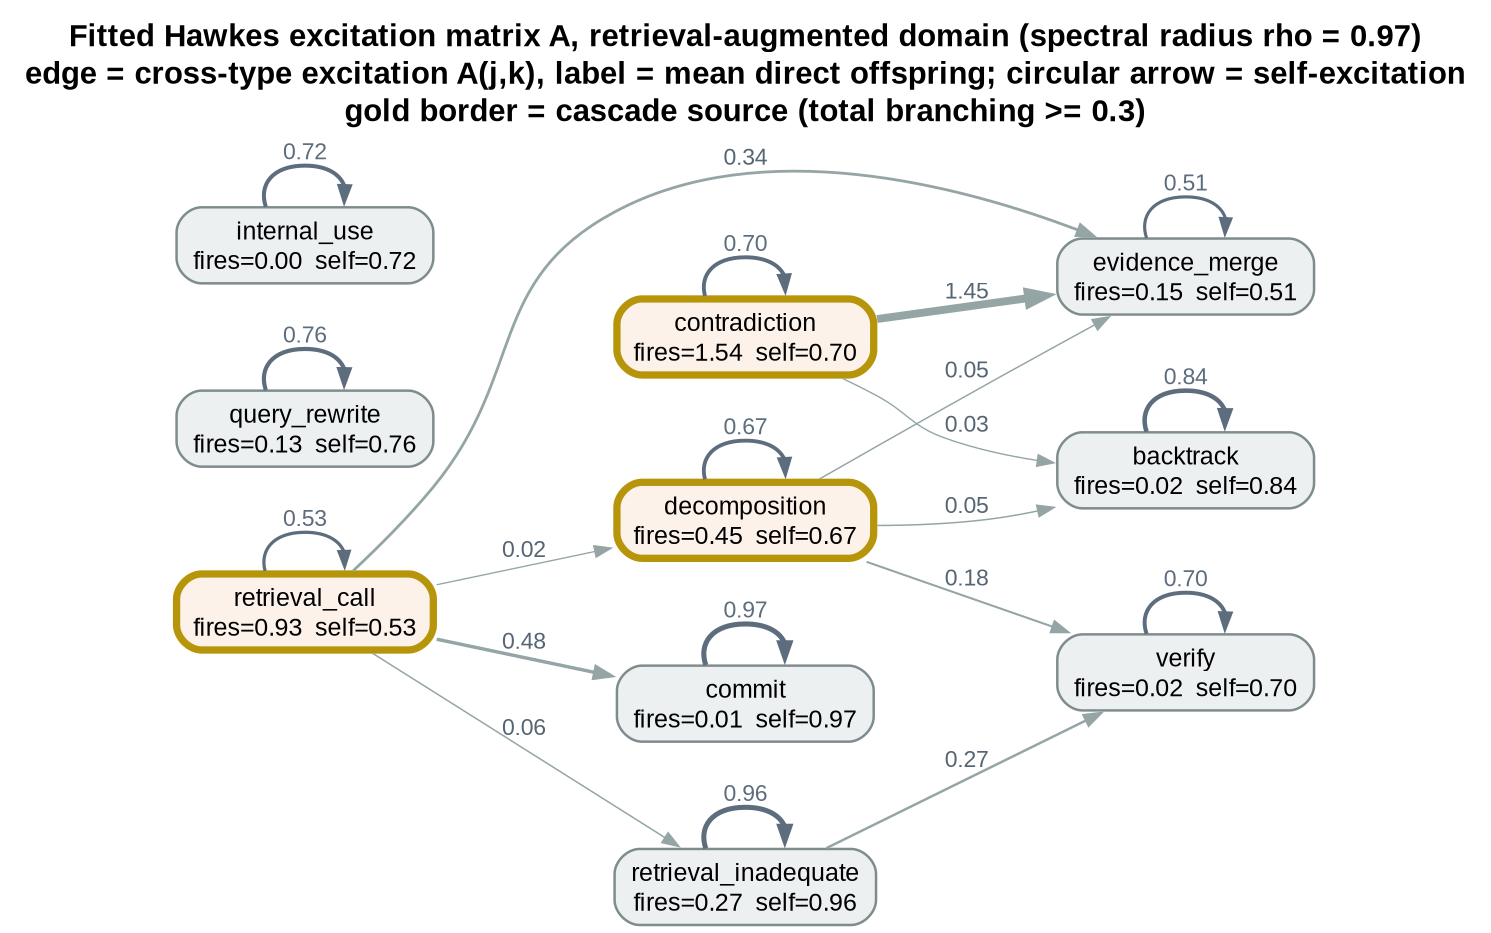
\includegraphics[width=0.8\textwidth]{fig_hawkes_R}
\caption{Связи между типами событий в поисковых трассах, оценённые с помощью процесса Хоукса. Число на ребре показывает, насколько событие у начала ребра повышает интенсивность события у его конца. Круговые стрелки показывают связь типа с самим собой. Спектральный радиус матрицы $A$ равен $0.973$. Величины следует читать как верхние границы из-за ошибок распознавателя событий.}
\label{fig:graph}
\end{figure}

\section{Модель событий и аналитические вмешательства}
\label{sec:theory}

Точечный процесс задаёт условное распределение будущих событий по уже наблюдённой части трассы. Мы используем его для двух задач: оценки будущего расхода и вычисления изменения ожидаемого расхода при гипотетическом ослаблении одного типа событий. Эта модель не выводит результат обучения с наградой, поскольку в ней нет параметров функции награды и оптимизации политики.

Пусть трасса представляет собой каскад событий с матрицей возбуждения $A=[A_{mk}]$, где $A_{mk}$ есть среднее число прямых потомков типа $k$, порождаемых одним событием типа $m$; событие типа $k$ стоит $c_k$ токенов; каскад начинается с событий, приходящих извне, со средним вектором $m_{\mathrm{imm}}$. Обозначим $R=(I-A)^{-1}$.

\begin{assumption}[субкритичность]\label{a1}
$\rho(A)<1$, где $\rho$ обозначает спектральный радиус, то есть наибольший модуль собственного числа матрицы $A$. Формулировать условие нужно именно через $\rho$, а не через норму: для матрицы $A$, оценённой по поисковым трассам, $\lVert A\rVert_\infty=2.23$ при $\rho(A)=0.973$.
\end{assumption}
\begin{theorem}[ожидаемый расход при прореживании событий]\label{thm:as}
При предположении~\ref{a1} и неотрицательных ограниченных стоимостях: (i) ожидаемый бюджет трассы равен $\mathbb E[B]=m_{\mathrm{imm}}^{\top}R\,c$, где $e_j^{\top}Rc$ есть ожидаемая стоимость каскада от одного события типа $j$; (ii) при прореживании потомства событий типа $k$ с вероятностью $\delta$, то есть $A(\delta)=A-\delta e_ke_k^{\top}A$, выполняется точное тождество ранга один
\begin{equation}
\mathbb E[B]-\mathbb E[B](\delta)=\frac{\delta\,\Lambda_k\;e_k^{\top}(R-I)\,c}{1+\delta\,(R_{kk}-1)}\ \ge 0,
\label{eq:sherman}
\end{equation}
где $\Lambda_k=\bigl(m_{\mathrm{imm}}^{\top}R\bigr)_k$ есть $k$-я компонента вектора $m_{\mathrm{imm}}^{\top}R$, то есть ожидаемое число событий типа $k$ за всю трассу до вмешательства; кроме того, $\rho(A(\delta))\le\rho(A)$.
\end{theorem}

Тождество показывает монотонное снижение ожидаемого расхода внутри линейной ветвящейся модели. Оно не связывает вес длины $\lambda$ с величиной прореживания $\delta$ и потому не является доказательством эффекта обучения. Для такой связи требуется сравнить параметры процесса до и после обучения либо случайно вмешаться в выбранный тип событий. Отметим и различие операций: тождество \eqref{eq:sherman} прореживает потомство событий типа $k$, то есть строку матрицы возбуждения, тогда как симуляционные вмешательства ниже домножают интенсивность типа, то есть столбец матрицы вместе с внешним притоком. Это разные вмешательства, и их эффекты сопоставляются только качественно.

\paragraph{Подтверждённые и неподтверждённые следствия рамки.} Мы проверили эти утверждения на $6{,}151$ трассе. Качественные следствия подтвердились: разброс расхода намного превышает средний расход, а очень большие расходы встречаются чаще, чем прогнозирует модель с постоянной вероятностью завершения после каждого следующего токена. Чем выше оценённая по данным способность каскада самоподдерживаться в паре $\langle$модель$\times$бенчмарк$\rangle$, тем чаще встречаются очень длинные трассы. Вероятность больших расходов приближённо убывает как степень; показатель этой степени падает с ростом способности каскада самоподдерживаться, ранговая корреляция равна $-0.69$ при $p=0.005$. Превышение разброса над средним, наоборот, растёт, ранговая корреляция равна $+0.67$ при $p=0.006$. Количественные следствия не подтвердились. Формула $\mathbb E[B]=m_{\mathrm{imm}}^{\top}Rc$, выведенная для каскада без ограничения по времени, завышает полное число потомков в $4$-$10$ раз, потому что ядра с параметрами, оценёнными по данным, затухают медленно и каскад не успевает закончиться в пределах трассы; та же формула, переписанная на конечный горизонт, попадает в наблюдаемые счётчики. Значение $\rho(A)=0.973$, полученное при оценивании матрицы, завышено: наблюдаемая частота очень длинных трасс соответствует значениям $0.75$-$0.9$. Само $\rho(A)$ по счётчикам событий восстановить нельзя, профиль правдоподобия по нему плоский; восстановить можно сумму авторегрессионных коэффициентов, приведённую в разделе~\ref{sec:labels}. Поэтому мы пользуемся тождествами в форме на конечный горизонт, значение $\rho(A)$, оценённое по событиям, принимаем за верхнюю границу и доверительных интервалов на нём не строим: вблизи единицы интервал вида среднее плюс минус отклонение оказывается пустым. Правило остановки, основанное на супермартингале Вилля, тоже требует осторожности: с оценённой, а не известной точно интенсивностью оно даёт слишком слабую защиту, доля эмпирических нарушений доходит до $0.35$ при номинальных $0.1$, и его приходится калибровать на отложенных трассах; после калибровки оно экономит $10$-$25\%$ токенов относительно прогона без него на тех парах $\langle$модель$\times$бенчмарк$\rangle$, где трассы длиннее всего.

\paragraph{Выбор типа события для вмешательства.} Аналитическое тождество \eqref{eq:sherman} мы дополнили оценкой по симуляции: обучили пошаговую модель, прогнозирующую по уже прошедшей части трассы тип следующего события, промежуток до него и момент завершения трассы, и прогнали через неё роллауты, домножая интенсивность выбранного типа события на заданный множитель. Устойчивую к смене разметки основу дают два эффекта: при переоценке на разметке модели-судьи эффект \textsf{commit} сохраняется и равен от $-0.10$ до $-0.13$ логарифма расхода на одно стандартное отклонение счётчика, и появляется эффект \textsf{failed\_attempt} от $+0.13$ до $+0.15$, поскольку разметка по шаблонам пропускает этот класс в $3$-$12$ раз. Остальные оценки разметко-зависимы. Ослабление \textsf{backtrack} вдвое сокращает ожидаемый расход математического домена почти вдвое, с $2{,}804$ до $1{,}431$ токена, и прогнозируемая доля правильных ответов при этом не падает, но на разметке судьи этот эффект не сохраняется, поэтому вмешательства в \textsf{backtrack} требуют эксперимента, в котором продолжение размышления навязывается случайно выбранным трассам. Усиление завершающего \textsf{commit} даёт то же сокращение расхода при наименьшем изменении интенсивности. В поисковом домене ослабление \textsf{query\_rewrite} вдвое сокращает расход с $1{,}676$ до $1{,}015$ токенов, то есть на $39\%$. Если вместо симуляции оценивать те же эффекты статической регрессией, не учитывающей обратную связь событий друг на друга, эффект \textsf{backtrack} занижается на порядок, так что обратную связь учитывать необходимо.

\paragraph{Распределение расхода между задачами.} Одинаковый потолок на каждую задачу расходует бюджет впустую: он обрывает трудную задачу, которой не хватило нескольких сотен токенов, тогда как соседние задачи той же группы заканчивают раньше и своего потолка не выбирают. Если одновременно обслуживается группа из $K$ запросов под общим бюджетом, искать надо распределение, максимизирующее ожидаемое число решённых задач при ограничении на сумму расходов. После замены каждой кривой завершения её вогнутой оболочкой задача становится линейной программой, которую решает жадное заполнение: на каждом шаге очередной токен выделяется задаче с наибольшим приростом вероятности успеха на один токен. Мы приводим эту конструкцию как предложение, а не как измеренный результат: на реально обслуживаемой группе запросов мы её не проверяли.

\section{Инструмент как рычаг расхода}
\label{app:tool}

Инструмент повышает долю правильных ответов, предотвращая обрывы по длине. Мы сравнили Qwen3.6 на $500$ вопросах MATH500 с доступом к исполнителю Python и без него при одинаковой температуре и потолке $7000$ токенов. Доля правильных ответов равна $0.940$ с инструментом и $0.890$ без него. Механизм прироста локализуется парным разбором. Среди $461$ вопроса, где обе версии завершились, после ручной проверки автоматического сравнения остаётся одно содержательное расхождение. Среди $34$ вопросов, где версия без инструмента не завершилась, версия с инструментом решила $27$, $p=7.5\cdot10^{-9}$. Поэтому инструмент повышает долю правильных ответов под ограничением, прежде всего переводя незавершённые ответы в завершённые, а не меняя исход среди уже завершённых пар.

На $437$ парах, правильно решённых обоими режимами, медиана парного сокращения расхода равна $872$ токенам при цене вызова $1.2$ токен-эквивалента, критерий Уилкоксона даёт $p<0.0001$. Маргинальные медианы равны $1204$ токена с инструментом и $2131$ без него, но парной оценкой служит именно разность $872$. Одним исполнением кода эту экономию объяснить нельзя. На $399$ вопросах, где модель вызвала Python, медианное парное сокращение равно $898$ токенам, а на $101$ вопросе без единого вызова оно равно $3082$ токенам. Режимы различаются не только наличием исполнителя, но и системным запросом, поэтому текущий опыт устанавливает эффект доступа к инструменту, но не разделяет влияние запроса и фактического исполнения кода. Для такого разделения нужен контроль с тем же системным запросом, но без переданного модели инструмента.

\bibliographystyle{acl_natbib}
\bibliography{references}

\end{document}
